\documentclass[12pt]{article}
\usepackage{amsmath, amssymb, amsthm}
\usepackage[margin=1in]{geometry}
\usepackage{natbib}
\usepackage{color}
\usepackage{hyperref}
\usepackage{graphicx}
\usepackage{booktabs}
\usepackage{multirow}
\usepackage{subcaption}

\newtheorem{theorem}{Theorem}
\newtheorem{proposition}{Proposition}
\newtheorem{corollary}{Corollary}
\newtheorem{remark}{Remark}

\newcommand{\RAH}{\mathrm{RAH}}
\newcommand{\RMST}{\mathrm{RMST}}
\newcommand{\DRMST}{D\text{-}\mathrm{RMST}}
\newcommand{\dd}{\,d}
\newcommand{\TauSim}{40}
\newcommand{\TauCM}{24}
\newcommand{\TBFading}{43}
\newcommand{\ScTauLight}{0.154}
\newcommand{\ScTauHeavy}{0.058}
\newcommand{\CoxHROriginal}{0.740}
\newcommand{\CoxHRSensitivity}{0.783}
\newcommand{\CoxPOriginal}{0.002}
\newcommand{\CoxPSensitivity}{0.052}
\newcommand{\DrmstOriginal}{1.75}
\newcommand{\DrmstSensitivity}{1.73}
\newcommand{\DrmstPOriginal}{0.012}
\newcommand{\DrmstPSensitivity}{0.058}
\newcommand{\RahOriginal}{0.739}
\newcommand{\RahSensitivity}{0.743}
\newcommand{\RahPOriginal}{0.003}
\newcommand{\RahPSensitivity}{0.014}
\newcommand{\AreDrmstCoxCM}{0.915}
\newcommand{\AreRahCoxCM}{1.199}
\newcommand{\AreRahDrmstCM}{1.310}
\newcommand{\EreDrmstCoxCM}{0.935}
\newcommand{\EreRahCoxCM}{1.332}
\newcommand{\EreRahDrmstCM}{1.425}
\newcommand{\CosSqCoxCM}{0.552}
\newcommand{\CosSqDrmstCM}{0.506}
\newcommand{\CosSqRahCM}{0.662}
\newcommand{\PowerCoxCM}{0.717}
\newcommand{\PowerDrmstCM}{0.680}
\newcommand{\PowerRahCM}{0.843}
\newcommand{\PowerCoxCMPct}{72}
\newcommand{\PowerDrmstCMPct}{68}
\newcommand{\PowerRahCMPct}{84}
\newcommand{\NPowerCoxCM}{400}
\newcommand{\NPowerDrmstCM}{400}
\newcommand{\NPowerRahCM}{300}
\newcommand{\NPowerCoxMorePct}{33}
\newcommand{\NPowerDrmstMorePct}{33}
\newcommand{\SchoenfeldPCM}{0.002}
\newcommand{\WeibullShapeControl}{1.264}
\newcommand{\WeibullScaleControl}{13.076}
\newcommand{\WeibullShapeTreatment}{0.987}
\newcommand{\WeibullScaleTreatment}{17.320}
\newcommand{\AlphaCMOne}{0.187}
\newcommand{\AlphaCMCross}{1.97}
\newcommand{\AlphaCMTau}{-0.693}
\newcommand{\SzeroCMTau}{0.12}
\newcommand{\AreRahCoxPHHeavyLowS}{0.798}
\newcommand{\AreRahDrmstPHHeavyLowS}{0.812}
\newcommand{\AreRahCoxPHShapeHalf}{0.922}
\newcommand{\AreRahCoxPHShapeTwo}{0.737}
\newcommand{\AreDrmstCMTauEighteen}{0.651}
\newcommand{\AreDrmstCMTauTwentyone}{0.789}
\newcommand{\AreDrmstCMTauTwentyfour}{0.915}
\newcommand{\AreRahCMTauEighteen}{1.198}
\newcommand{\AreRahCMTauTwentyone}{1.211}
\newcommand{\AreRahCMTauTwentyfour}{1.199}
\newcommand{\AreRahDrmstCMTauEighteen}{1.841}
\newcommand{\AreRahDrmstCMTauTwentyfour}{1.310}
\newcommand{\AreDrmstCMDropoutLow}{0.884}
\newcommand{\AreDrmstCMDropoutHigh}{1.039}
\newcommand{\AreRahCMDropoutLow}{1.180}
\newcommand{\AreRahCMDropoutHigh}{1.265}
\newcommand{\AreRahDrmstCMDropoutLow}{1.335}
\newcommand{\AreRahDrmstCMDropoutHigh}{1.217}
\newcommand{\AreDrmstCMPH}{0.995}
\newcommand{\AreRahCMPH}{0.870}
\newcommand{\AreEreNearOneBand}{0.07}

\newcommand{\xmeng}[1]{\textcolor{red}{[xmeng: {#1}]}}
\newcommand{\ken}[1]{\textcolor{orange}{[Ken: {#1}]}}
\newcommand{\hajime}[1]{\textcolor{blue}{[Hajime: {#1}]}}
\newcommand{\lu}[1]{\textcolor{green}{[Lu: {#1}]}}

\title{A Cosine-Projection Framework for Choosing Among\\
       Cox HR, D-RMST, and Average-Hazard Tests in Survival Trials}
\author{Xiang Meng, Lu Tian, Hajime Uno}
\date{\today}

\begin{document}
\maketitle

\begin{abstract}
Three summary statistics are available for comparing two
survival distributions, the hazard ratio (HR) from Cox model, the difference in restricted mean survival time (D-RMST), and the ratio of average hazards
(RAH), yet they detect different patterns of treatment effect with different efficiency, and there is no guidance on
which to use in a given trial.  RAH, in particular, is a recent
proposal, whose large-sample efficiency has not been studied systematically. In the paper, we show that all three statistics admit a first-order weighted comparison
of cumulative hazard functions, represent each statistic by a direction in
$L^2([0,\tau],\lambda_0(v)\dd v)$, and establish that its asymptotic
efficiency relative to the oracle test is exactly the squared cosine of the
angle between that direction and the true signal for the treatment effect; the asymptotic relative efficiency of any two tests is then a ratio of squared cosines.
Because the censoring and accrual design enters only through the at-risk
weight function $w(v)$, the cosine metric explains---and predicts---how design
choices can reverse the efficiency ordering among tests, something raw
weight-function plots cannot do, and it doubles as a design-stage
diagnostic for test selection.
We illustrate the framework using the CheckMate~057 immunotherapy trial and
corroborate the theoretical results through simulations spanning proportional- and
non-proportional-hazards settings.
\end{abstract}

\section{Introduction}
\label{sec:intro}


Three tests are available for comparing two survival distributions in
randomized clinical trials, and they occupy very different positions in
practice.
The test based on Cox proportional hazards model (or the log-rank test) is the only one in widespread use: it is
optimal under proportional hazards (PH) assumption and remains the default for
regulatory submissions.
The test based on restricted mean survival time (RMST) \citep{Uno2014} is
used increasingly often when the proportional hazards assumption is
violated, offering a clinically interpretable estimand---the difference
in restricted mean survival time (D-RMST) up to a horizon $\tau$.
Unlike D-RMST, the ratio of average hazards (RAH) \citep{Uno2023} is an estimand on the \emph{rate} scale: it contrasts the two arms' average event rates per unit of event-free person-time on a time window. As D-RMST, RAH also doesn't require PH assumption.


Being relatively new, the RAH-based test is also much less well understood than the other two tests. Although its null distribution is known \citep{Uno2023}, its large-sample \emph{efficiency}—that is, its power and the alternatives against which it is most sensitive, relative to the two established tests—has not been systematically studied. This is important because practitioners often face a practical question: \emph{given a specific trial design and an anticipated treatment-effect pattern, which test is most appropriate?}



CheckMate 057 was a randomized, open-label Phase III trial comparing nivolumab with docetaxel in 582 patients with previously treated non-squamous NSCLC \citep{Borghaei2015}. The primary endpoint was overall survival. Individual-level data were reconstructed from the published Kaplan--Meier (KM) curves using the algorithm of \cite{Guyot2012}.
We considered two reconstructed datasets, both comprising $n_0=290$ docetaxel and $n_1=292$ nivolumab patients, that differed only in their censoring patterns. In the ``\emph{original}'' dataset, the subject-level data were reconstructed from the published figure and the reported riskset information, yielding 419 observed events (226 in the docetaxel group and 193 in the nivolumab group). To illustrate the dependence of test results on the censoring-time distribution, we reconstructed a second dataset with the same marginal KM curves as those reported in the publication but different risk-set sizes over time. This results in only 267 observed events (134 in the docetaxel group and 133 in the nivolumab group). The time window of interest was set to $[0,\tau]=[0,24]$ months.


Table~\ref{tab:results-cm057-intro} presents the results of the three aforementioned tests for both reconstructed datasets. The point estimates are broadly consistent between the two datasets (Cox HR: \CoxHROriginal\ vs.\ \CoxHRSensitivity; D-RMST: \DrmstOriginal\ vs.\ \DrmstSensitivity\ months; RAH: \RahOriginal\ vs.\ \RahSensitivity), all indicating a survival advantage for nivolumab. In contrast, the corresponding $p$-values differ substantially (Cox model-based test: $p=\CoxPOriginal$ vs.\ $p=\CoxPSensitivity$; D-RMST-based test: $p=\DrmstPOriginal$ vs.\ $p=\DrmstPSensitivity$; RAH-based test: $p=\RahPOriginal$ vs.\ $p=\RahPSensitivity$). Thus, the $p$-values for the Cox model- and D-RMST-based tests cross the conventional 0.05 threshold between the two analyses, whereas the RAH-based test remains statistically significant in both datasets. This sensitivity to the censoring distribution does not indicate a failure of any particular test. Rather, it reflects a fundamental interplay among the underlying treatment-effect pattern, the choice of test, and the censoring distribution. Understanding and quantifying this interplay is the central objective of this paper.



The motivating example raises a question that is more general than
``is RAH better than D-RMST?''. Instead, the correct question is

\begin{quote}
\emph{Given assumed survival functions, a treatment-effect pattern, and
a censoring/accrual design, which test---Cox, D-RMST, or RAH---is most
statistically efficient?}
\end{quote}




\begin{table}[ht]
\centering
\caption{CheckMate 057 overall-survival results under two censoring reconstructions. All three methods use an analysis horizon of $\tau=24$ months; for Cox, follow-up is administratively censored at $\tau$ before model fitting. Values below 1 for Cox and RAH, or above 0 for D-RMST, favor nivolumab.}
\label{tab:results-cm057-intro}
\begin{tabular}{lcccc}
\toprule
Dataset & Method & Estimate & 95\% CI & $p$-value
\\
\midrule
Original & Cox & 0.740 & (0.609, 0.898) & 0.002 \\
Original & D-RMST & 1.75 & (0.39, 3.11) & 0.012 \\
Original & RAH & 0.739 & (0.604, 0.902) & 0.003 \\
Sensitivity & Cox & 0.783 & (0.612, 1.003) & 0.052 \\
Sensitivity & D-RMST & 1.73 & (-0.06, 3.53) & 0.058 \\
Sensitivity & RAH & 0.743 & (0.586, 0.942) & 0.014 \\
\bottomrule
\end{tabular}
\end{table}


\subsection{Related work}
\label{sec:related}

Reservations about the HR as a summary measure of treatment effect are long-standing. When the PH assumption is violated, the Cox maximum partial-likelihood estimator converges to a weighted average of the time-varying log hazard ratio, with weights depending on the study-specific censoring distribution \citep{Cox1972,Hernan2010,Horiguchi2019}. Consequently, two trials with the same underlying biological treatment effect can report materially different HRs simply because their accrual rates or follow-up durations differ. Moreover, because the HR is a relative measure without a direct absolute reference, it can be difficult to translate into clinically actionable terms \citep{Uno2014}. These concerns have motivated estimands defined directly through the marginal survival function, such as the D-RMST \citep{Royston2013,Uno2014,Tian2014,survRM2} and RAH \citep{Uno2023,meng2026efficient}.

Efficiency comparisons among these tests have received much less attention. The closest antecedent to the present paper is \citet{Tian2018}, who compare the logrank test with the D-RMST test through their asymptotic relative efficiency under both PH and non-PH settings. They find that the D-RMST test performs nearly as well as the logrank test when PH holds and can substantially outperform it when PH fails, whereas the logrank test retains an advantage when the two survival curves separate only late in follow-up. When the underlying alternative is unknown, combination (Max-combo) tests trade a small amount of efficiency for greater robustness by considering a family of tests \citep{LinEtal2020}.




\subsection{Contributions and Paper Outline}
\label{sec:contributions}

This paper makes three contributions. First, we characterize the large-sample efficiency of the RAH-based test and place it on a common Pitman-efficacy scale with the Cox- and D-RMST-based tests, extending \citet{Tian2018}. Second, we show that each test's efficiency relative to the oracle test equals the squared cosine of the angle between its test direction and the signal direction, so that any pairwise ARE is a ratio of squared cosines. Third, because censoring and accrual enter only through the at-risk weight $w(\cdot)$, we use the cosine metric to show how design choices can reverse the efficiency ordering and to select a test at the design stage. All results are supported by extensive numerical studies, including simulations and an analysis of the reconstructed CheckMate~057 trial.

The paper is organized as follows. Section~\ref{sec:setup} defines the three test statistics, shows that each can be expressed as a form of weighted logrank test statistic, and presents their asymptotic efficiency under local alternative. Section~\ref{sec:cosine} develops the cosine metric for facilitating the comparison of the three tests. Section~\ref{sec:sim} presents simulation studies under a range of settings, and Section~\ref{sec:cm057-analysis} reports statistical analysis for a study design based on CheckMate~057 trial. Section~\ref{sec:discussion} summarizes the main contributions and discusses directions for future research.

\section{Three Statistics, a Weighted-Log-Rank Representation, and Their Efficiency}
\label{sec:setup}

\subsection{Setup and notation}
\label{sec:notation}

Let $T_k$ ($k=0,1$) denote the event time in group $k$ with survival
function $S_k(t)$, cumulative hazard function $\Lambda_k(t)$, and hazard function $\lambda_k(t)$.
Define
\begin{equation}
  F_k(t)=1-S_k(t)\qquad \mbox{and} \qquad R_k(t)=\int_0^t S_k(u)\dd u.
\end{equation}
Thus, $F_k(t)=\Pr(T_k\le t)$ is the cumulative incidence rate (the probability
that the event has occurred by time $t$) and $R_k(\tau)$ is the RMST on $(0,\tau]$.
Let $C_k$ be the censoring time, independent of $T_k$, with
$G_k(t)=\Pr(T_k\wedge C_k\ge t)$ bounded away from zero on $(0,\tau]$.
Let $p_k$ be the limiting proportion of subjects in group $k$ $\left(p_0+p_1=1\right)$.
Lastly, the at-risk weight function is defined as
\begin{equation}\label{eq:w}
  w(t)=\frac{p_0\,p_1\,G_0(t)\,G_1(t)}{p_0\,G_0(t)+p_1\,G_1(t)}.
\end{equation}

Two simplifying conditions recur throughout the paper.
By \emph{equal allocation} we mean a balanced design with $p_0=p_1=1/2.$
By \emph{a common censoring distribution} we mean that the two groups
share the same marginal censoring law, and we write
$S_C(v)=\Pr(C\ge v)$ for the common censoring survival function;
this is the case for administrative censoring.
Under these two conditions, the at-risk weight \eqref{eq:w} becomes $w(t)=0.5\times S_C(t)/\{S_0(t)^{-1}+S_1(t)^{-1}\}.$ If the null hypothesis, $S_1(t)=S_0(t), t\in [0, \tau],$ is also true, then  the weight function further reduces to $w(t)=S_0(t)S_C(t)/4$.



\subsection{The three test statistics}
\label{sec:three-stats}

We can test $H_0:S_1(t)=S_0(t), t\in [0, \tau]$ against alternatives using three
statistics.  For each statistic, we state the corresponding estimand, point estimator, and asymptotic distribution of the test statistic.
Throughout, $\hat S_k(\cdot)$ and
$\hat\Lambda_k(\cdot)$ denote the Kaplan--Meier and Nelson--Aalen estimators of
$S_k(\cdot)$ and $\Lambda_k(\cdot)$, respectively, $\hat G_k(\cdot)$ denote the empirical counterpart of $G_k(\cdot)$, and $\hat{R}_k(t)$ denote $\int_0^t \hat{S}_k(u)du$, a consistent estimator of $R_k(t).$


\paragraph{HR.}
Under the PH assumption,
$$\theta=\log\left\{\frac{\lambda_1(t)}{\lambda_0(t)} \right\}$$
 does not depend on $t$ and can be consistently estimated by the maximum partial likelihood estimator $\hat{\theta}.$ As $n\to \infty,$
\[
  \sqrt n(\hat\theta-\theta)\xrightarrow{d}N(0,\sigma_\theta^2),
\]
where
\begin{equation}\label{eq:var-cox}
  \sigma_\theta^2
    =\left\{\int_0^{\tau}
       \frac{e^{\theta}p_0p_1\,G_0(u)\,G_1(u)}
            {p_0\,G_0(u)+e^{\theta}p_1\,G_1(u)}\,\dd\Lambda_0(u)
      \right\}^{-1}.
\end{equation}
Under $H_0:\lambda_1(\cdot)=\lambda_0(\cdot)$,
$$\sigma_\theta^2=\left\{\int_0^{\tau}w(u)\dd\Lambda_0(u)\right\}^{-1},$$
 and the
Wald statistic
\(
  Z_{\mathrm{Cox}}
    =\sqrt n\,\hat\theta/\hat\sigma_\theta
\)
is asymptotically standard normal, where $\hat{\sigma}_\theta^2$ is a consistent estimator of $\sigma_\theta^2.$

 We use $Z_{\rm Cox}$ for all numerical studies in this paper, whereas its theoretical properties were examined based on an asymptotically equivalent score statistic, i.e., the
log-rank statistic. The details are given in Section~\ref{sec:wlr} and Appendix~\ref{sec:appendix-weights}.

\paragraph{D-RMST.}
The \textbf{D-RMST} test is based on the difference between two estimated RMSTs:
\begin{equation}\label{eq:rmst-stat}
  \hat\theta_{\DRMST}=\hat R_1(\tau)-\hat R_0(\tau)
            =\int_0^\tau\bigl[\hat S_1(t)-\hat S_0(t)\bigr]\dd t,
\end{equation}
the area between the two Kaplan--Meier curves up to $\tau$
\citep{Uno2014,survRM2}. Let $\theta_{\DRMST}=R_1(\tau)-R_0(\tau)$ be the true RMST difference. It is a clinically interpretable estimand, and oftentimes preferred when the PH assumption may be violated.  Then, $\hat\theta_{\DRMST}$ is a consistent estimator of $\theta_{\DRMST}$ and
$\sqrt{n}(\hat\theta_{\DRMST}-\theta_{\DRMST})
\xrightarrow{d}N(0,\sigma_{\DRMST}^2)$ with
\begin{equation*}\label{eq:var-rmst}
  \sigma_{\DRMST}^2
    =\sum_{k=0}^{1}
     \int_0^\tau\!\left\{\int_v^\tau S_k(u)\dd u\right\}^{\!2}
     \frac{\dd\Lambda_k(v)}{p_k\,G_k(v)},
\end{equation*}
as $n \to \infty$
\citep{Tian2018}. Under the null, the Wald statistic
\(
  Z_{\DRMST}
    =\sqrt n\,\hat{\theta}_{\DRMST}/\hat\sigma_{\DRMST}
\)
is asymptotically standard normal, where $\hat{\sigma}_{\DRMST}^2$ is a consistent estimator of $\sigma_{\DRMST}^2.$

\paragraph{RAH.}
The AH for group $k$ on $(0,\tau]$ is
\begin{equation*}\label{eq:AH}
  \eta_k(\tau)=\frac{F_k(\tau)}{R_k(\tau)}
              =\int_0^\tau\lambda_k(t)\,
               \frac{S_k(t)}{\int_0^\tau S_k(u)\dd u}\dd t,
\end{equation*}
a weighted average of hazard function over $[0, \tau]$ \citep{Uno2023}.
$\eta_k(\tau)$ is a population-level person-time event rate.
Two properties make
AH attractive as a robust summary on the hazard scale.  First, $\eta_k(\tau)$ is defined purely through the event-time distribution
and is therefore not affected by the censoring distribution. On the other hand, the commonly used person-time incidence rate $\Pr(T\le C)/\mathbb{E}(T\wedge C)$ depends on both survival and censoring distributions \citep{Uno2023}.
Second, AH respects stochastic ordering: if $S_1(t)\ge S_0(t)$ for all
$t\le\tau$, then $\eta_1(\tau)\le\eta_0(\tau)$.
The ratio of AH (RAH) between two groups is
\begin{equation}\label{eq:RAH}
  \theta_{\RAH}
    =\frac{\eta_1(\tau)}{\eta_0(\tau)}
    =\frac{F_1(\tau)/R_1(\tau)}{F_0(\tau)/R_0(\tau)},
\end{equation}
with $\theta_{\RAH}=1$ under $H_0$.  Its estimator $\hat\theta_{\RAH}$ can be obtained by
replacing $F_k(\tau)$ and $R_k(\tau)$ with $1-\hat{S}_k(\tau)$ and $\hat R_k(\tau)$ in \eqref{eq:RAH}, respectively. As $n \to \infty$, $\sqrt{n}(\log\hat\theta_{\RAH}-\log\theta_{\RAH})\xrightarrow{d}N(0,\sigma_{\RAH}^2)$, \citep{Uno2023},
where
\begin{equation}\label{eq:var-RAH}
  \sigma_{\RAH}^2
    =\sum_{k=0}^{1}
     \int_0^\tau
     \!\left\{\frac{1}{F_k(\tau)}-\frac{R_k(u)}{R_k(\tau)}\right\}^{\!2}
     \frac{\dd\Lambda_k(u)}{G_k(u)\,p_k}.
\end{equation}
The test statistic $Z_{\RAH}=\sqrt{n}\log(\hat\theta_{\RAH})/\hat\sigma_{\RAH}$
is asymptotically $N(0,1)$ under $H_0$, where $\hat{\sigma}_{\RAH}^2$ is a consistent estimator of $\sigma^2_{\RAH}.$

\subsection{Weighted-log-rank representation}
\label{sec:wlr}

All three statistics, to the first order, can be written as a weighted contrast of
Nelson--Aalen cumulative-hazard estimates from two groups:
\begin{equation}\label{eq:wlr-generic}
  U_W=\int_0^\tau W(t)d\hat{\Delta}_\Lambda(t),
\end{equation}
 where
\[
  \hat{\Delta}_\Lambda(v)=\hat\Lambda_1(v)-\hat\Lambda_0(v).
\]
Under $H_0,$ the two cumulative hazards coincide and $U_W$ has mean zero. The
weight $W(\cdot)$ decides which time periods contribute to the comparison, and
choosing $W(\cdot)$ to match the anticipated alternative is the classical route to
constructing powerful, distribution-free survival tests \citep{FlemingHarrington1991,Tian2018}. Rigorous arguments for expressing three aforementioned test statistics in this form can be found in Appendix~\ref{sec:appendix-weights}.

\paragraph{HR.}
The log-rank statistic, the score statistic under Cox model, can be written as
\begin{equation}\label{eq:cox-stat}
  U_{\mathrm{Cox}}
    =\int_0^\tau \frac{p_1p_0\hat{G}_1(t)\hat{G}_0(t)}{p_1\hat{G}_1(t)+p_0\hat{G}_0(t)}
     d\hat{\Delta}_\Lambda(t).
\end{equation}
 Under
the local alternatives considered in section \ref{sec:efficiency}, a one-step expansion of the score function from the partial likelihood function around $\theta=0$ yields that
$\sqrt n\,\hat\theta=\sigma_\theta^2\sqrt n\,U_{\mathrm{Cox}}+o_p(1)$. Thus, the Wald statistic,  $Z_{\mathrm{Cox}}$ and the normalized $\sqrt{n}U_{\mathrm{Cox}}$ are asymptotically equivalent. Furthermore,
the random weight in \eqref{eq:cox-stat} converges to at-risk weight $w(\cdot)$ in
\eqref{eq:w} in probability, as $n \to \infty,$

\paragraph{D-RMST and RAH.}
Neither statistic is a log-rank type statistic by construction, but each is a
smooth functional of $\hat\Lambda_1(\cdot)$ and
$\hat\Lambda_0(\cdot)$.
For D-RMST, $R(\Lambda)=\int_0^\tau \exp\{-\Lambda(t)\}\dd t$, and
\begin{align*}
\hat{\theta}_{\DRMST}
=&\int_0^\tau S_0(t)\left[\exp\left\{-\hat{\Delta}_\Lambda(t)\right\}-1\right]\dd t+O\bigl(\|\hat{\Delta}_\Lambda\|^2\bigr)\\
=& -\int_0^\tau S_0(t)\,\hat{\Delta}_\Lambda(t)\dd t +O\bigl(\|\hat{\Delta}_\Lambda\|^2\bigr)\\
=&-\int_0^\tau \left\{R_0(\tau)-R_0(t)\right\}d\hat{\Delta}_\Lambda(t)+O\bigl(\|\hat{\Delta}_\Lambda\|^2\bigr) \\
=&-U_{\DRMST}+O_p\bigl(n^{-1}\bigr)
\label{eq:drmst-expansion}
\end{align*}
under local alternative. As the remainder is $O_p(n^{-1})$, $Z_{\DRMST}$ and the normalized $\sqrt{n}U_{\DRMST}$ are asymptotically equivalent.  RAH can be handled the same way, with an extra delta-method step for the ratio $F_k(\tau)/R_k(\tau)$, and
\begin{align*}
\log(\hat{\theta}_{\RAH})=& \int_0^\tau \left[\frac{S_0(\tau)}{F_0(\tau)}
              +\frac{ R_0(\tau)-R_0(t)}{R_0(\tau)}\right]d\hat{\Delta}_\Lambda(t)+O\bigl(\|\hat{\Delta}_\Lambda\|^2\bigr)\\
              =& U_{\RAH}+O_p(n^{-1})
\end{align*}
under local alternative. As a result, $Z_{\RAH}$ and the normalized $\sqrt{n}U_{\RAH}$ are asymptotically equivalent.

All $U_X$ are oriented so that $U_X<0$ indicates benefit of treatment (hence $U_{\DRMST}=-\hat\theta_{\DRMST}$ to first order); since $\xi_X$ depends on $\mu_X^2$, the orientation does not affect efficiency.

\medskip
In summary, under equal allocation and a common censoring assumption, the
resulting weights for $U_{\mathrm Cox}$, $U_{\DRMST}$ and $U_{\RAH}$ are
\begin{align*}
  W_{\mathrm{Cox}}(t)
    &=\;S_0(t)\,S_C(t)/4,\\
  W_{\DRMST}(t)
    &= R_0(\tau)-R_0(t), \mbox{ and}\\
  W_{\RAH}(t)
    &= \left[\frac{S_0(\tau)}{F_0(\tau)}
              +\frac{ R_0(\tau)-R_0(t)}{R_0(\tau)}\right],
\end{align*}
respectively. Since multiplying the weight function by any nonzero constant yields an equivalent test statistic, without loss of generality, we may use following equivalent weight functions
\begin{align*}
  W_{\mathrm{Cox}}(t)=&S_0(t)\,S_C(t)\\
  W_{\DRMST}(t)=&\frac{ R_0(\tau)-R_0(t)}{R_0(\tau)}\\
  \mbox{ and }~
  W_{\RAH}(t)=&S_0(\tau)+\left\{1-S_0(\tau)\right\}W_{\DRMST}(t)
\end{align*}
for three test statistics.
On the current scale, all three weights equal $1$ at $t=0$, their limits at
$t=\tau$ are $S_0(\tau)S_C(\tau)$, $0$, and $S_0(\tau)$. Also, weight for $U_{\RAH}$ is a simple linear transformation of that for $U_{\DRMST}$.

The Cox model-based log-rank weight tracks the amount of information in the risk set. It is the largest early in follow-up, when the risk set is large, and decreases over time as deaths and censoring deplete the risk set. Under the PH assumption, this weighting is optimal. The D-RMST weight represents the RMST within the window \([t, \tau]\). It also places greater weight on earlier follow-up, which decreases monotonically to zero at \(\tau\), thereby also down-weighting survival differences in late follow-up. The weight for RAH is likewise monotone decreasing, but remains strictly positive at \(\tau\), and therefore places relatively greater emphasis on late-stage survival differences than the weight function for D-RMST. This common representation allows us to formally examine the test efficiency in the next section.





\subsection{Asymptotic efficiency}
\label{sec:efficiency}

To compare the three tests on a single scale we use the
\emph{Pitman efficacy}, the standard local-power measure for asymptotically
normal tests \citep{Pitman1949}.  Following \citet{Tian2018}, we embed the
two-sample problem in a sequence of contiguous (local) alternatives indexed
by a fixed log-hazard-ratio shape $\alpha(\cdot)$ on $(0,\tau]$,
\begin{equation}\label{eq:local-alt-main}
  H_{An}:\qquad
  \log\!\left\{\frac{\lambda_{1n}(t)}{\lambda_0(t)}\right\}
    =\frac{\alpha(t)}{\sqrt{n}},
\end{equation}
so that the two hazards coincide as $n\to\infty,$ while the between-group difference is in the order of $O(1)$.  Under \eqref{eq:local-alt-main}, for
test $X\in\{\mathrm{Cox},\DRMST,\RAH\},$ the test statistic is asymptotically normal, i.e.,
\begin{equation*}
  \sqrt{n}\,U_X\xrightarrow{d}N\!\bigl(\mu_X,\;\sigma_X^2\bigr),
\end{equation*}
where
\begin{equation*}
  \mu_X=\int_0^\tau W_X(t)\,\alpha(t)\,\lambda_0(t)\dd t
  \qquad\mbox{and}\qquad
  \sigma_X^2=\int_0^\tau \frac{W_X(t)^2}{w(t)}\,\lambda_0(t)\dd t .
\end{equation*}
The drift $\mu_X$ is obtained by substituting
$\sqrt n \hat\Delta_{\Lambda}(t)$ by $\alpha(t)\lambda_0(t)$ in \eqref{eq:wlr-generic}. The variance $\hat{\sigma}_X^2$ is the null variance of
\eqref{eq:wlr-generic}.
The \emph{asymptotic efficiency} (AE), or Pitman
efficacy, of test $X$ is the squared standardized drift
\begin{equation}\label{eq:efficacy-def}
  \xi_X=\frac{\mu_X^2}{\sigma_X^2},
\end{equation}
which governs the local power. The derivation of $\mu_X$ for RAH-based test can be found in Appendix \ref{sec:appendix-proofs}. Furthermore, the
explicit expressions of
$\xi_{\mathrm{Cox}},$ $\xi_{\DRMST}$ and $\xi_{\RAH}$ are provided in Appendix \ref{sec:appendix-pitman}.
The \emph{asymptotic relative efficiency} (ARE) of test $X$ versus test $Y$
is the ratio of corresponding AEs:
\begin{equation}\label{eq:are-def}
  \mathrm{ARE}(X,Y)=\frac{\xi_X}{\xi_Y},
\end{equation}
which approximates the inverse ratio of the sample sizes the two tests
require to reach the same local power against \eqref{eq:local-alt-main};
$\mathrm{ARE}(X,Y)>1$ means that test $X$ is more efficient and needs proportionally fewer subjects than $Y$ \citep{Tian2018,Pitman1949}.  Because ARE may be a poor proxy for the sample size ratio in finite-sample setting, we also report the \emph{empirical relative efficiency} (ERE), the
ratio of squared standardized effect sizes estimated by simulation (Section~\ref{sec:sim}),
\begin{equation}\label{eq:ere-def}
  \mathrm{ERE}(X,Y)
    =\frac{E(U_X)^2/\mathrm{Var}(U_X)}
          {E(U_Y)^2/\mathrm{Var}(U_Y)},
\end{equation}
with the expectations and variances approximated by their Monte Carlo averages in simulation
\citep{Tian2018}.


\section{The geometric interpretation of AE}
\label{sec:cosine}
Section~\ref{sec:wlr} reduced all three tests to the weighted logrank test~\eqref{eq:wlr-generic} and showed that their AE depends on the test only through the weight function.  This is the basis
of the classical comparison of \citet{Tian2018}, who contrast the Cox and
D-RMST tests by inspecting their weight functions $W_{\mathrm{Cox}}(\cdot)$ and
$W_{\DRMST}(\cdot)$ directly. In this section, we replace the side-by-side weight comparison with a geometric quantity, a cosine, turning AE into an angle in a function space.


\subsection{Signal direction and test direction}
\label{sec:directions}

Suppose that all candidate statistics are evaluated on the same horizon $\tau$, and consider the function space $L^2([0,\tau], \lambda_0(v)\dd v)$, where the inner product
\begin{equation}\label{eq:inner-product}
  \langle f,g\rangle=\int_0^\tau f(v)\,g(v)\,\lambda_0(v)\dd v,
 \end{equation}
and norm $\|f\|^2=\langle f,f\rangle .$ Next, we
define the \emph{signal direction} for local alternative $\alpha(\cdot)/\sqrt{n}$ and \emph{test direction} for test $X\in\{\mathrm{Cox},\DRMST,\RAH\}$, as
\begin{equation}\label{eq:directions}
  s_\alpha(t)=\alpha(t)\sqrt{w(t)}\qquad \mbox{and} \qquad
  h_X(t)=\frac{W_X(t)}{\sqrt{w(t)}},
\end{equation}
respectively.

The signal direction, $s_\alpha(t),$ describes where the detectable treatment effect is by combining the local log-HR representing the underlying between-group difference at $t$ and $\sqrt{w(t)}$ representing the amount of information available to detect the difference at time $t$.  Thus, $s_\alpha(t)$ is large where the true effect is big and sufficient information is available to detect it. It is a ``direction'' since only its shape over $t$, not its overall magnitude, matters. The test direction, $h_X(t)=W_X(t)/\sqrt{w(t)},$ is the analogous
object built from the test's own weight.  $W_X(\cdot)$ records where the test is
prepared to look for the effect. $\sqrt{w(t)}$ in the denominator ensures that $h_X(t)$ represents test weight per unit of information available at time $t$. Next, we have
\[
  \langle s_\alpha,h_X\rangle
    =\int_0^\tau \alpha(t)\sqrt{w(t)}\,\frac{W_X(t)}{\sqrt{w(t)}}\,
      \lambda_0(t)\dd t
    =\int_0^\tau W_X(t)\,\alpha(t)\,\lambda_0(t)\dd t=\mu_X,
\]
\[
  \|h_X\|^2
    =\int_0^\tau \frac{W_X(v)^2}{w(v)}\,\lambda_0(v)\dd v=\sigma_X^2 ,
\]
Consequently the AE \eqref{eq:efficacy-def}
\begin{equation}\label{eq:eff-inner}
  \xi_X=\frac{\langle s_\alpha,h_X\rangle^2}{\|h_X\|^2}.
\end{equation}

\subsection{The cosine metric}
\label{sec:cosine-metric}

Writing the inner product in \eqref{eq:eff-inner} as

$$
\langle s_\alpha,h_X\rangle=\|s_\alpha\|\,\|h_X\|\cos(\theta_X),
$$
or equivalently,
\begin{equation}\label{eq:eff-cos}
\cos^2(\theta_X)=\frac{\langle s_\alpha,h_X\rangle^2}
{\|s_\alpha\|^2\|h_X\|^2}
=\frac{\xi_X}{\|s_\alpha\|^2},
\end{equation}
where \(\theta_X\) denotes the angle between the signal direction \(s_\alpha\) and the test direction \(h_X\). Intuitively, \(\theta_X\) measures the mismatch between where the test places its weight and where the detectable treatment effect is concentrated: a small \(\theta_X\) indicates good alignment and  high local power. The quantity \(\|s_\alpha\|^2\) is the AE of the oracle test using the optimal weight \(\alpha(t)w(t)\). Therefore, $\cos^2(\theta_X)$ is the ARE of test \(X\) relative to the oracle test, $O$. In general, the ARE of test $X$ vs test $Y$ can be expressed as
\begin{equation}\label{eq:are-cosine}
  \mathrm{ARE}(X, Y)=\frac{\cos^2(\theta_X)}{\cos^2(\theta_Y)}=\frac{\mathrm{ARE}(X, O)}{\mathrm{ARE}(Y, O)}.
\end{equation}



\medskip
As a preview, Figure~\ref{fig:cosine-geometry} provides geometric representations for three data-generating processes considered in \citep{Tian2018}. Specifically, the left column displays \(s_\alpha(t)\), \(h_{\mathrm{Cox}}(t)\), \(h_{\mathrm{DRMST}}(t)\), and \(h_{\mathrm{RAH}}(t)\), whereas the right column depicts the corresponding directions on a compass, with the signal direction fixed at 12 o'clock and each test's \(\cos^2\theta_X\) shown at the tip of the corresponding arrow for test direction. More detailed results are presented in Section~\ref{sec:sim}.


\begin{figure}[ht]
  \centering
  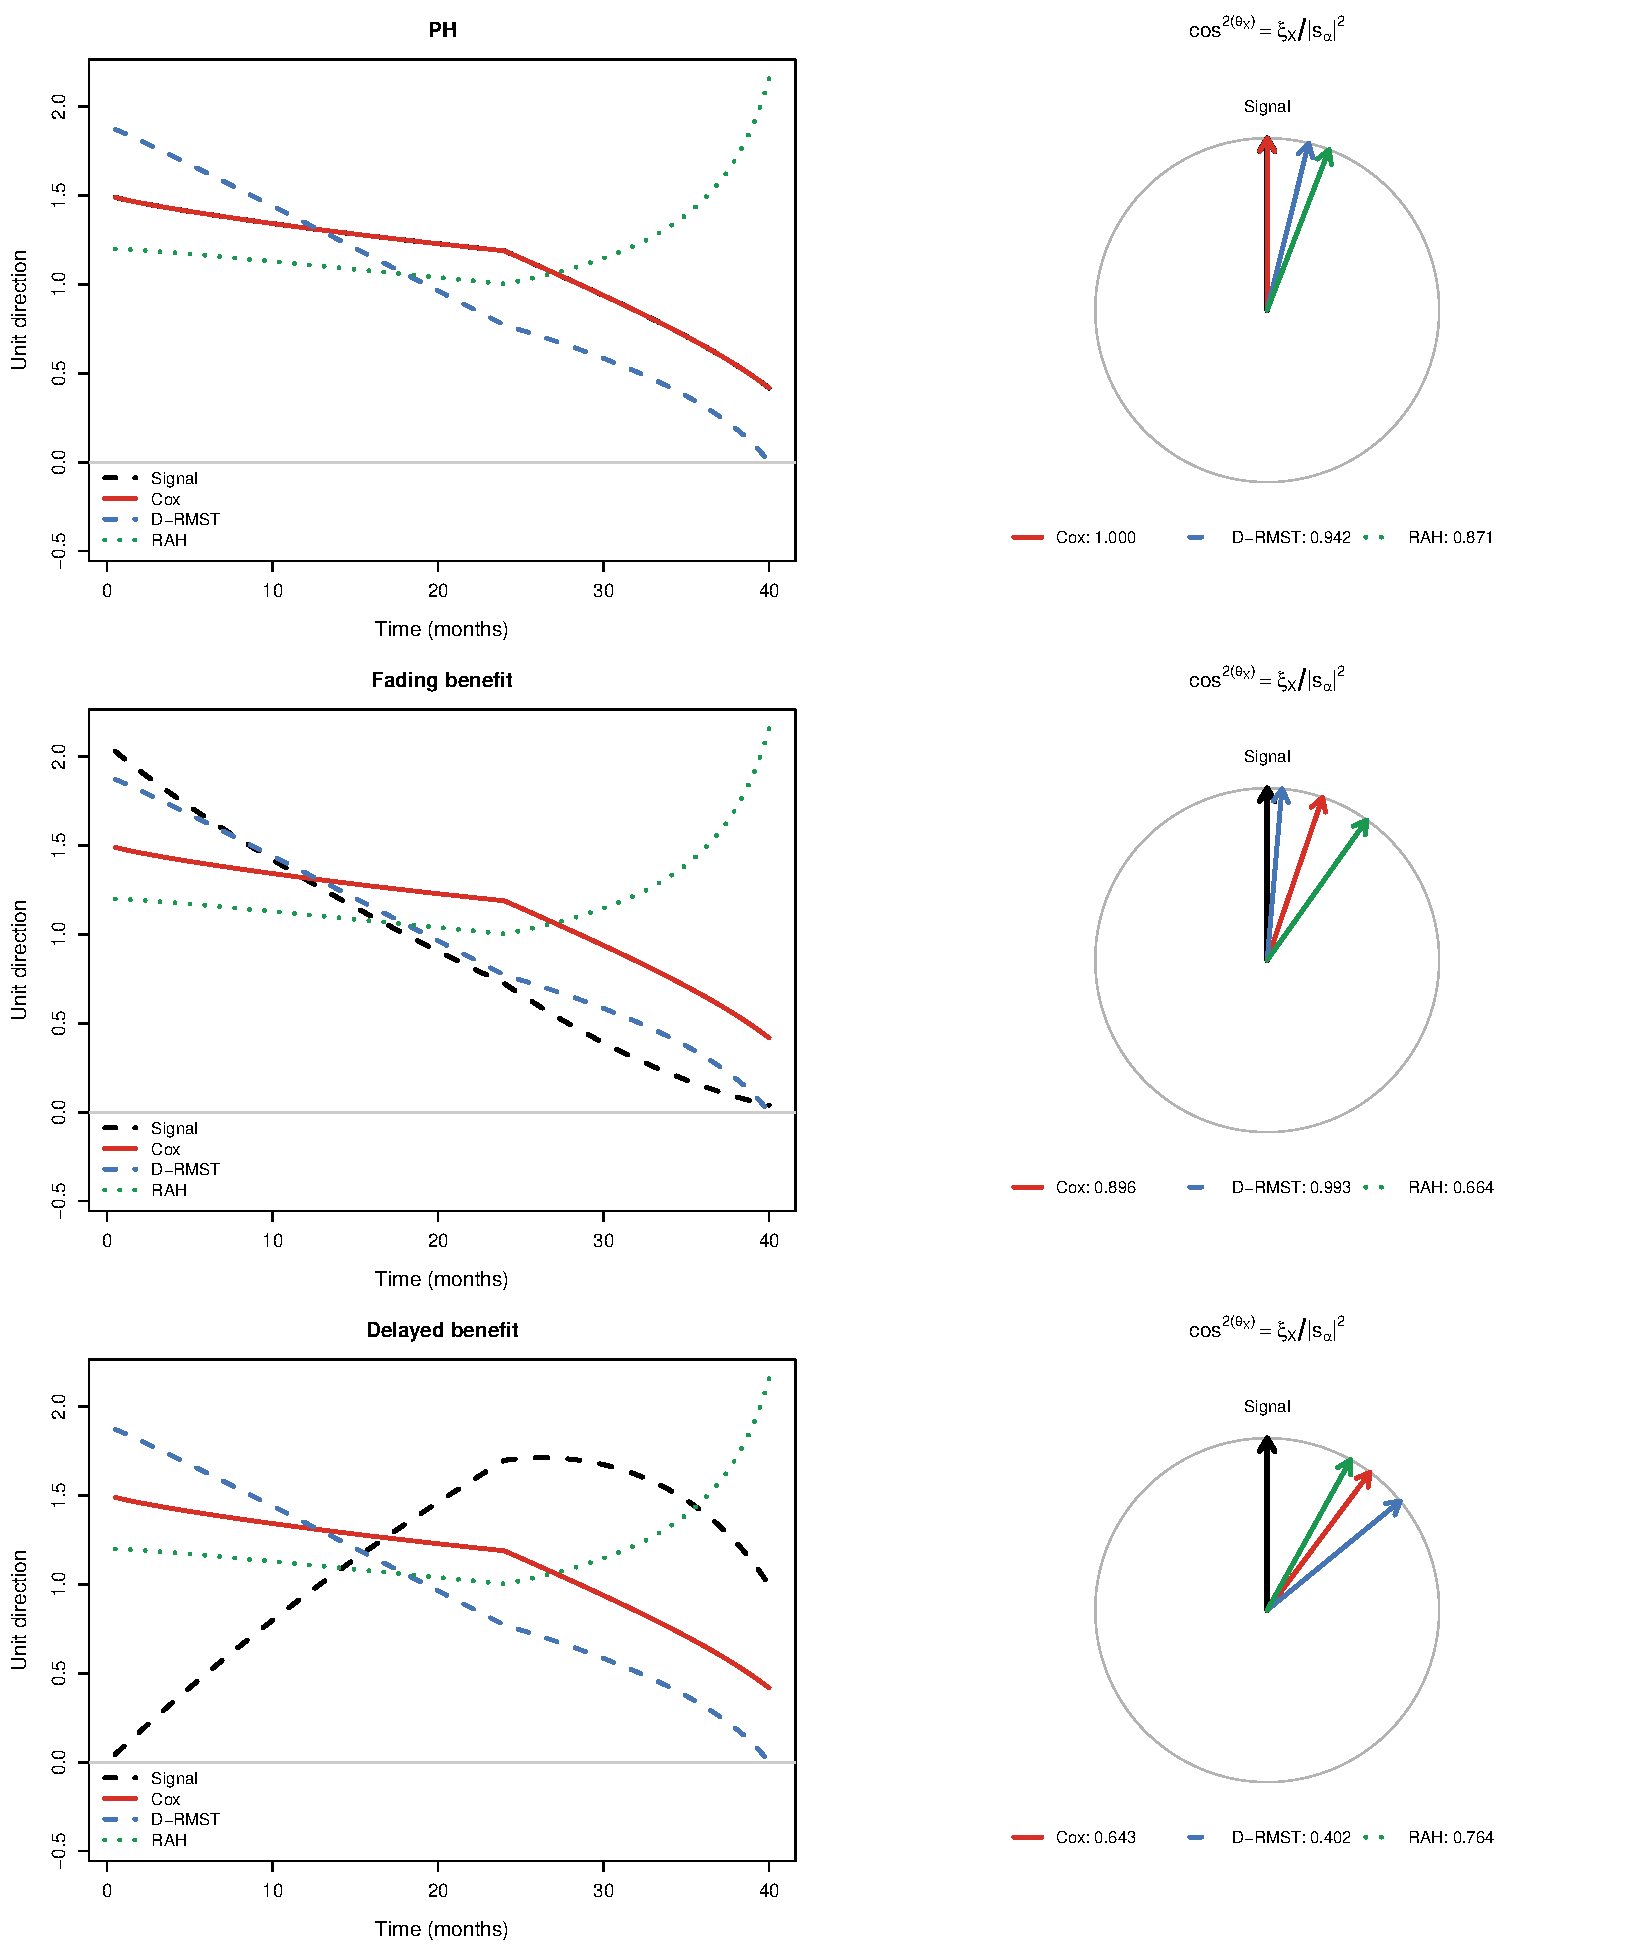
\includegraphics[width=0.95\linewidth]{output/figures/figure1-cosine-geometry.pdf}
  \caption{Unit-vector functions (left column) and compass diagrams
  (right column) for three scenarios
  (Weibull baseline: $\kappa=0.826$, $S_0(40)=0.50$, light censoring).
  The D-RMST and RAH tests are evaluated at
  $\tau=40$ months;
  Signal direction is placed at 12 o'clock in the
  compass diagrams; each test arrow is annotated with its $\cos^2(\theta_X)$ value.
  Under PH (top), Cox is aligned, while D-RMST and RAH lose some efficiencies.
  Under delayed benefit (bottom), the signal rotates toward the RAH
  direction, raising $\cos^2(\theta_{\RAH})$ above
  $\cos^2(\theta_{\mathrm{Cox}})$.}
  \label{fig:cosine-geometry}
\end{figure}

The cosine metric naturally applies at the trial design stage. Suppose that one has access to:
\begin{itemize}
\item assumed survival functions $S_0(t)$ and $S_1(t)$;
\item assumed treatment-effect $\alpha(t)$ (e.g., PH, delayed
benefit, et al.);
\item planned censoring and accrual distribution (which affects $w(\cdot)$); and
\item a set of test statistics.
\end{itemize}
Given these inputs, one can compute the signal and test directions and $\cos^2(\theta_X)$ for each candidate test and select the test with the highest $\cos^2(\theta_X)$, the one most aligned with the expected signal. Crucially, censoring and accrual are part of trial design and affect the value of $\cos^2(\theta_X).$ By varying $S_C(t)$, one can trace how the cosine metric changes and understand whether the selected test is robust to design assumptions. We demonstrate this in Section~\ref{sec:cm057-analysis} for CheckMate~057, and specifically trace the preferred test across design choices in a sensitivity analysis.




\section{Simulation Study}
\label{sec:sim}

\subsection{Design}
\label{sec:sim-design}

We compare the Cox, D-RMST, and RAH-based tests via ARE and ERE using the
same data-generating process of \citet{Tian2018}.
The baseline event-time distribution is Weibull($\kappa$, $\eta_0$)
with scale parameter $\eta_0$ chosen so that $S_0(\TauSim)$ equals a specified target survival rate at $\tau=\TauSim$ months and the default shape parameter $\kappa=0.826$ yielding a decreasing hazard
$\lambda_0(t)\propto t^{-0.174}$.
Censoring time $C=\min(E,U)$, where $E\sim\mathrm{Exp}(\lambda_c)$ and
$U\sim\mathrm{Uniform}(24,43)$ represent loss of follow-up and random entry, respectively. Two rates $\lambda_c\in\{0.0006,0.025\}$ for $E$
yield light ($S_C(\TauSim)=\ScTauLight$) and heavy ($S_C(\TauSim)=\ScTauHeavy$)
censoring.
Sample size $n_0=n_1=400$ per arm; $B=2000$ replicates are used for each simulation. We consider the following alternatives:

\noindent\textbf{PH scenario (Case 1):}
The event-time distribution in the treatment group is Weibull$(\kappa, \eta_1)$, where $\eta_1=\eta_0/0.70^{1/\kappa}$ yields a HR of 0.70. $\eta_0$ is adjusted so that
$S_0(40)=0.10,\ldots,0.80$ and 0.9.

\medskip
\noindent\textbf{Non-PH scenarios:}
$\kappa=0.826$ and
$S_0(40)=0.50$ for control subjects. The log-HR $\alpha(t)=\log[\lambda_1(t)/\lambda_0(t)]$
follows two patterns:
\begin{itemize}
  \item \textbf{Case~2 (fading benefit):}
    $\alpha(t)=-c_0\max(\TBFading-t,\,0)^s, s\in \{0.5, 1, 2\}$.
    The treatment benefit is the biggest early and fades to null at month \TBFading.
  \item \textbf{Case~3 (delayed benefit):}
    $\alpha(t)=-c_0t^s,  s\in \{0.5, 1, 2\}$.
    The treatment benefit is absent at $t=0$ and increases over follow-up.
\end{itemize}
In both cases $c_0>0$ is selected so that the mean log-HR over $[0,\tau]$ is approximately $\log(0.70)$. For Cases 2 and 3,  event-times in treatment arm are generated by numerical inversion of the cumulative hazard, i.e., $T_1 \sim \Lambda^{-1}_1\{\mbox{Exp}(1)\}.$

Figures~\ref{fig:dgp-ph}, \ref{fig:dgp-case2}, and~\ref{fig:dgp-case3}
display the survival curves and HRs for three
cases.
Each figure uses a four-panel layout: the top-left panel shows
$\exp\{\alpha(t)\}$ (the HR), and the
remaining panels show $S_0(t)$ (control, solid) against $S_1(t)$
(treatment, dashed) for different values of $s$.


Three simulation settings are also studied:
\begin{enumerate}
\item the PH setting with a HR=0.82 (Appendix ~\ref{sec:appendix-hr082});
\item the PH setting with alternative baseline survival distributions (Weibull$(\kappa, \eta_0)$ with \(\kappa=0.7, 1\) and 1.5), sample size (150 per arm), and trial horizon $(\tau=10)$ month (Appendix~\ref{sec:appendix-tau10});
\item the crossing-hazard setting with $\alpha(t)=\log(0.46)+(t/43)$ (the HR begins below~1 and rises to 1.25 at month 43) (Appendix~\ref{sec:appendix-crossing}).
\end{enumerate}

\medskip
\begin{figure}[ht]
  \centering
  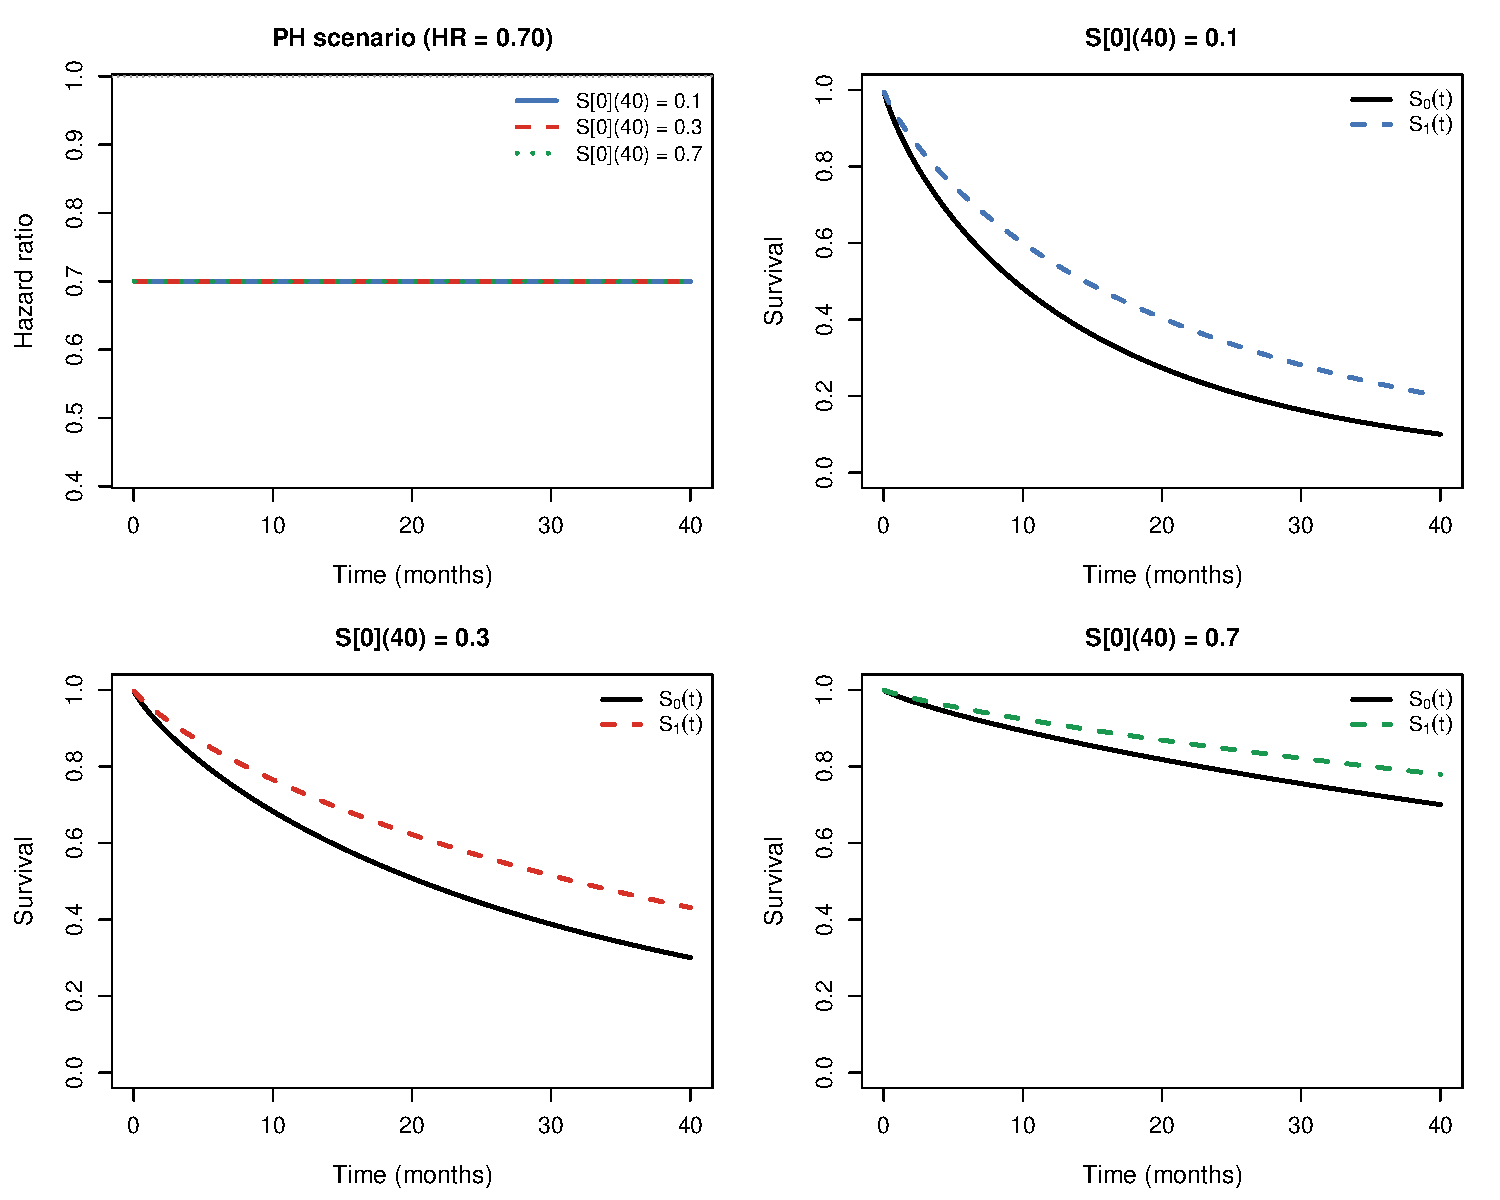
\includegraphics[width=0.95\linewidth]{output/figures/figure2-dgp-ph.pdf}
  \caption{\textbf{PH scenario} (HR $= 0.70$) and
    $S_0(\tau)\in\{0.10, 0.30, 0.70\}$.
    The HR is flat at 0.70; higher event rates produce greater absolute separation between two survival curves.}
  \label{fig:dgp-ph}
\end{figure}

\begin{figure}[ht]
  \centering
  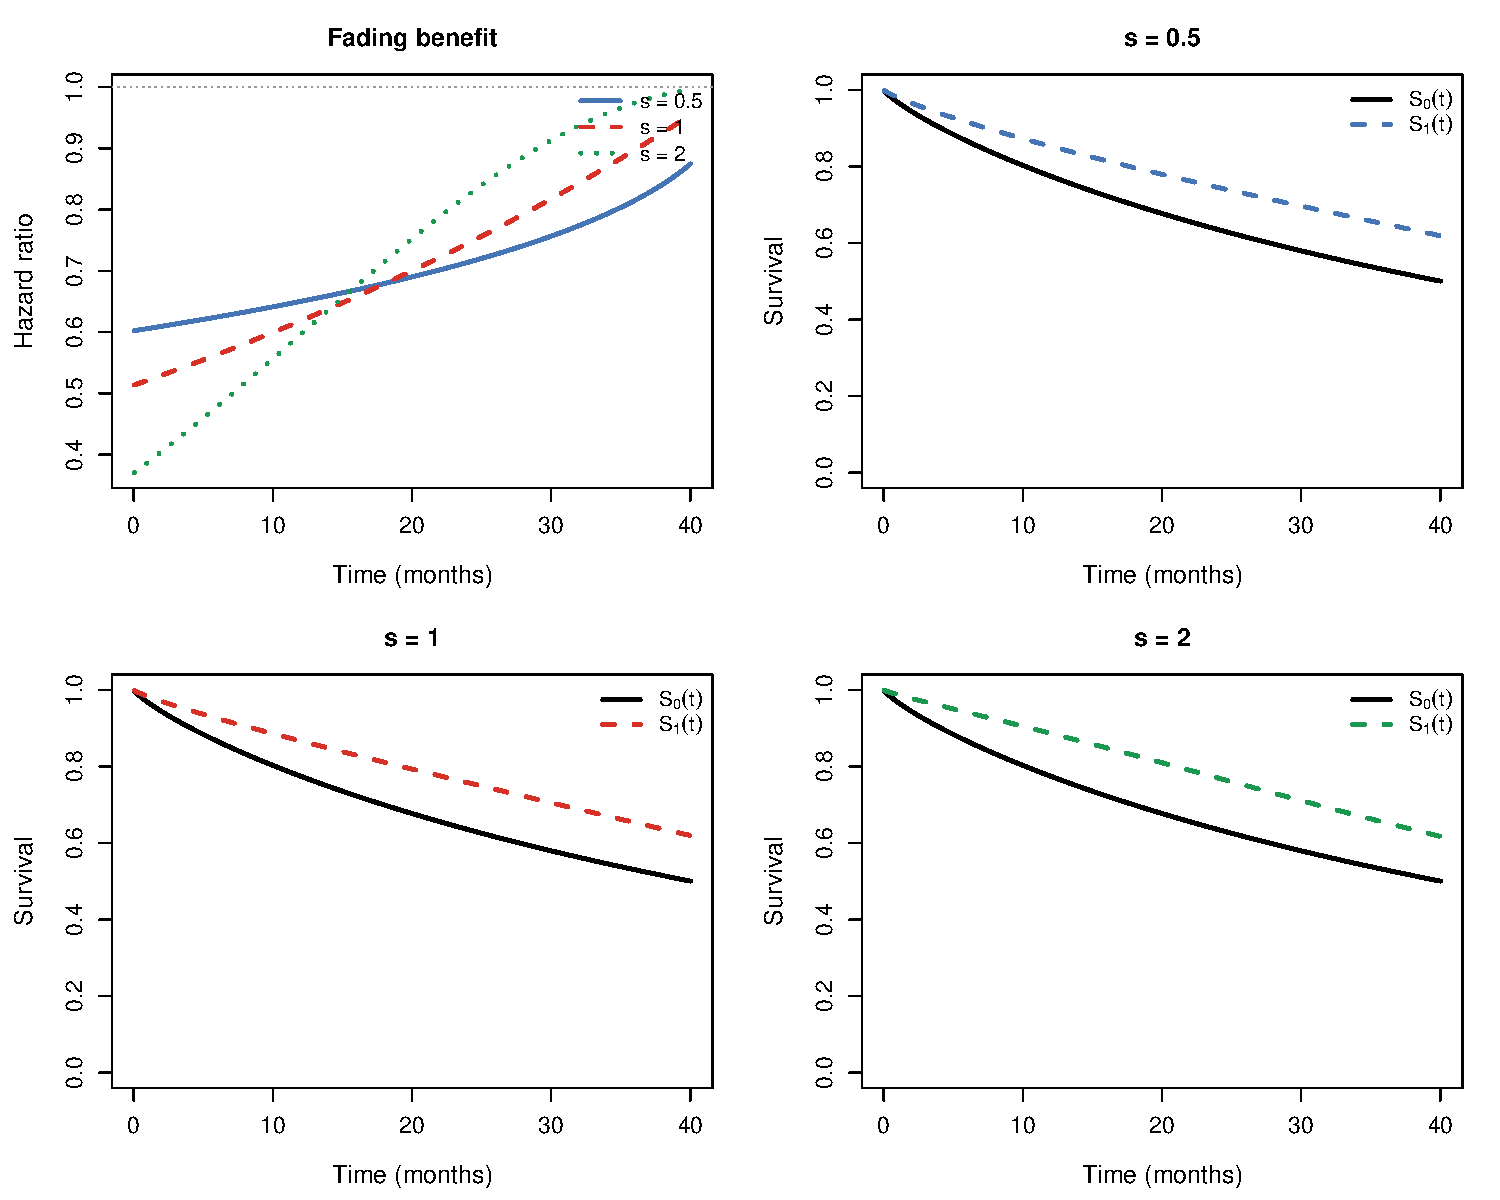
\includegraphics[width=0.95\linewidth]{output/figures/figure3-dgp-fading.pdf}
  \caption{\textbf{Case~2: fading benefit.}
    $\alpha(u)=-c_0\,\max(t_M-u,0)^s$,  mean log-HR $=\log(0.70)$.
    The HR is below 1 early and converges to 1 by $t_M$; larger $s$
    concentrates the benefit closer to $u=0$.}
  \label{fig:dgp-case2}
\end{figure}

\begin{figure}[ht]
  \centering
  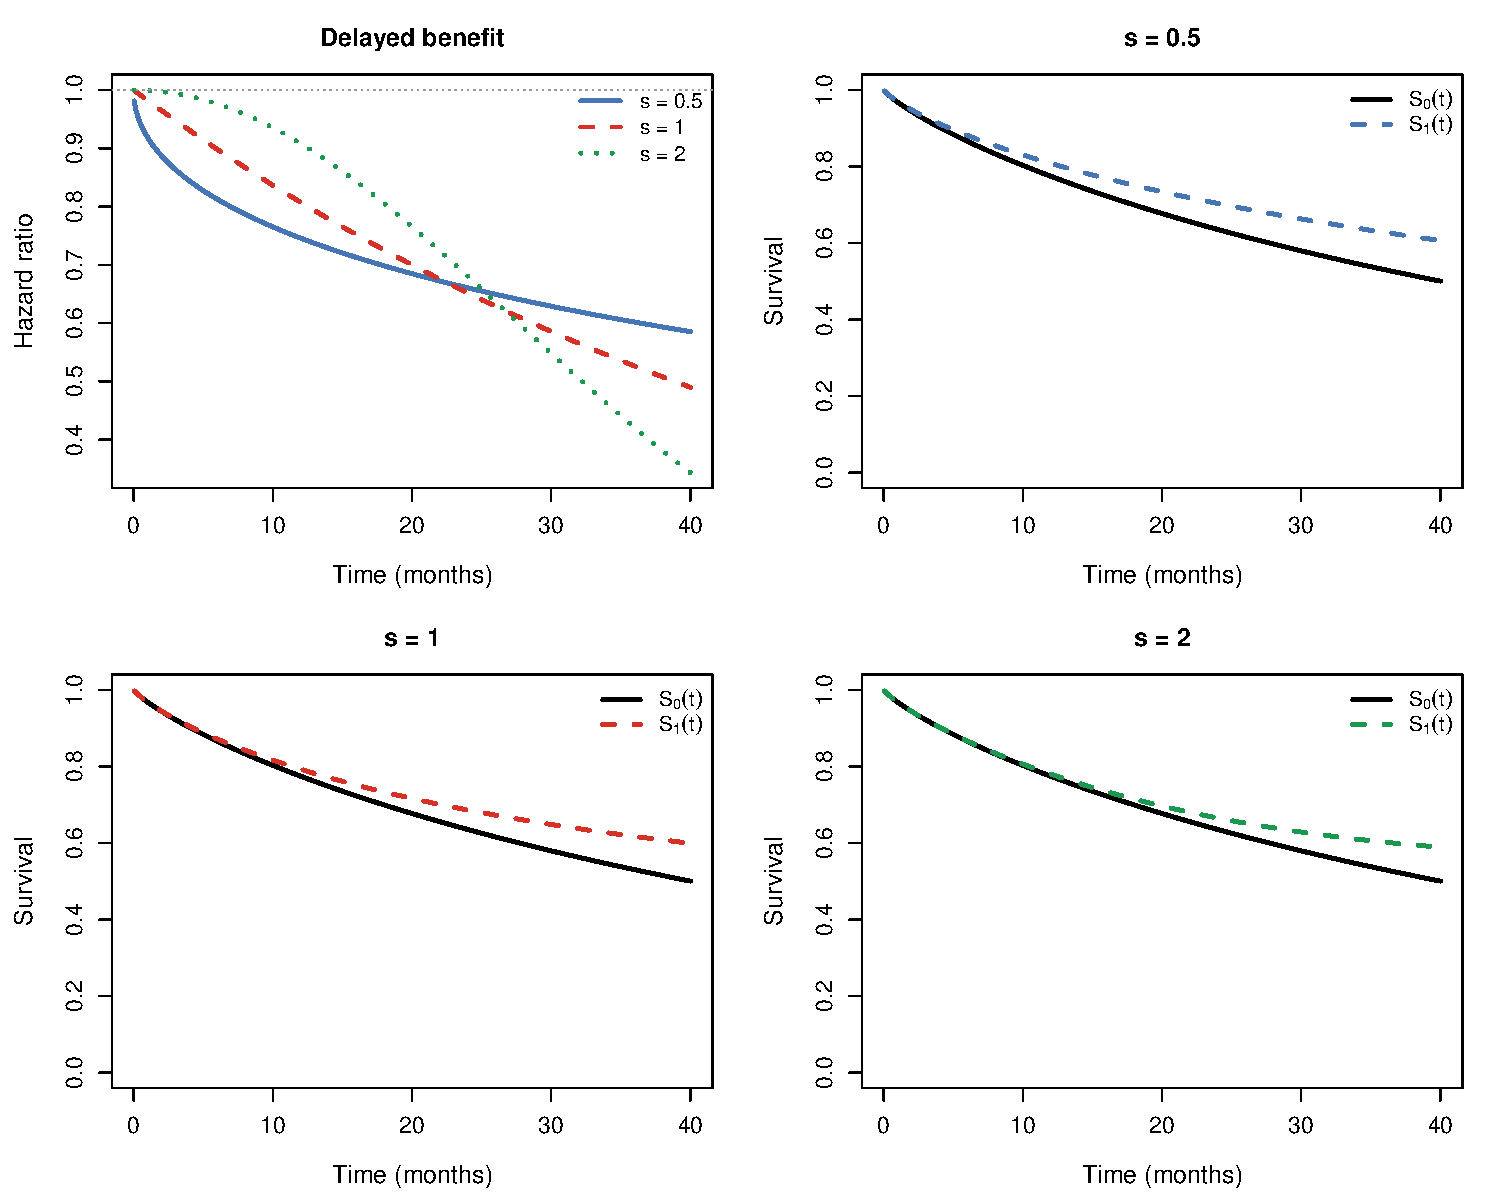
\includegraphics[width=0.95\linewidth]{output/figures/figure4-dgp-delayed.pdf}
  \caption{\textbf{Case~3: delayed benefit.}
    $\alpha(u)=-c_0\,u^s$, mean log-HR $=\log(0.70)$.
    The HR starts at 1 and decreases; larger $s$ delays the onset of the
    treatment effect, with the benefit concentrated at later time points for $s=2$.}
  \label{fig:dgp-case3}
\end{figure}

\subsection{PH scenario (Case 1)}
\label{sec:sim-ph}

Table~\ref{tab:main-sim-ph-hr070-s0-010-090-light-heavy} summarizes the comparison for \(S_0(40)\in\{0.10,\ldots,0.90\}\), \(\kappa=0.826\), and \(\mathrm{HR}=0.70\). Under light censoring, the ARE of the D-RMST-based test relative to Cox decreases gradually as \(S_0(40)\) increases. Under heavy censoring, however, this ARE remains close to 1 across the full range of \(S_0(40)\).

The ARE of the RAH-based test relative to the Cox model-based test is also below 1 throughout. This is expected as the Cox model-based test is optimal under the PH assumption. The efficiency declines as \(S_0(40)\) increases and more strongly under heavy censoring. As \(S_0(\tau)\) increases, the lower bound
$W_{\RAH}(\tau)=S_0(\tau)$ becomes larger, so that $
h_{\RAH}(\tau)=2
\sqrt{S_0(\tau)/S_C(\tau)}$
also increases. This inflates \(\|h_{\RAH}\|^2\) and enlarges RAH's discrepancy from the optimal test direction. At \(S_0(40)=0.10\) under heavy censoring, ARE(RAH/Cox) is \AreRahCoxPHHeavyLowS, whereas ARE(RAH/D-RMST) is \AreRahDrmstPHHeavyLowS. The ordering
$$
\mathrm{Cox}\ge \RAH \approx \DRMST
$$
under PH with light censoring and small \(S_0(\tau)\) is also evident geometrically in Figure~\ref{fig:cosine-geometry} (top row): the signal direction is aligned with the Cox model-based test direction, whereas the RAH and D-RMST test directions are more off-axis.

The ARE of the RAH-based test relative to the D-RMST-based test is close to 1 under light censoring but substantially lower under heavy censoring, indicating a more pronounced performance separation between the two procedures.



Table~\ref{tab:main-sim-ph-hr070-kappa-050-200-light-heavy} reports results for \(S_0(40)=0.50\) and \(\kappa\in\{0.5,0.826,1,1.5,2\}\). Under light censoring, the ARE of the RAH-based test relative to the Cox model-based test decreases from \AreRahCoxPHShapeHalf\ when \(\kappa=0.5\), corresponding to a decreasing baseline hazard, to \AreRahCoxPHShapeTwo\ when \(\kappa=2\), corresponding to an increasing baseline hazard. Intuitively, an increasing hazard shifts more events toward later follow-up, where RAH weighting differs more substantially from optimal weighting of Cox model-based test, thereby reducing its efficiency.

Both Tables~\ref{tab:main-sim-ph-hr070-s0-010-090-light-heavy} and~\ref{tab:main-sim-ph-hr070-kappa-050-200-light-heavy} show systematically larger efficiency losses for the RAH-based test under heavy censoring than under light censoring. This pattern persists across alternative baseline survival distributions and trial horizons.

In summary, these results show that the ARE of the competing tests depends materially on the censoring distribution. The censoring and accrual patterns induced by the study design should not be viewed merely as nuisance features; rather, they are important design inputs for choosing testing procedures.


\begin{table}[ht]
\centering
\caption{ARE and ERE under PH (HR$=0.70$), $\kappa=0.826$, $\tau=40$, $n=400$ per arm, $B=2000$.}
\label{tab:main-sim-ph-hr070-s0-010-090-light-heavy}
\resizebox{\textwidth}{!}{
\begin{tabular}{lccccccc}
\toprule
Censoring & $S_0(40)$ & ARE(D/C) & ARE(R/C) & ARE(R/D) & ERE(D/C) & ERE(R/C) & ERE(R/D)
\\
\midrule
Light & 0.10 & 0.994 & 0.941 & 0.947 & 1.007 & 0.946 & 0.940 \\
Light & 0.30 & 0.967 & 0.898 & 0.929 & 0.978 & 0.860 & 0.879 \\
Light & 0.50 & 0.942 & 0.871 & 0.924 & 0.948 & 0.893 & 0.942 \\
Light & 0.70 & 0.920 & 0.851 & 0.924 & 0.912 & 0.866 & 0.950 \\
Light & 0.90 & 0.901 & 0.835 & 0.927 & 0.919 & 0.832 & 0.905 \\
\midrule
Heavy & 0.10 & 0.982 & 0.798 & 0.812 & 0.997 & 0.725 & 0.727 \\
Heavy & 0.30 & 0.997 & 0.720 & 0.722 & 1.020 & 0.691 & 0.677 \\
Heavy & 0.50 & 0.998 & 0.680 & 0.682 & 1.024 & 0.671 & 0.656 \\
Heavy & 0.70 & 0.995 & 0.654 & 0.658 & 1.011 & 0.677 & 0.670 \\
Heavy & 0.90 & 0.990 & 0.635 & 0.642 & 1.019 & 0.658 & 0.646 \\
\bottomrule
\end{tabular}
}
\end{table}




\begin{table}[ht]
\centering
\caption{ARE and ERE under PH (HR$=0.70$), $S_0(40)=0.50$, $\tau=40$, $n=400$ per arm, $B=2000$.}
\label{tab:main-sim-ph-hr070-kappa-050-200-light-heavy}
\resizebox{\textwidth}{!}{
\begin{tabular}{lccccccc}
\toprule
Censoring & $\kappa$ & ARE(D/C) & ARE(R/C) & ARE(R/D) & ERE(D/C) & ERE(R/C) & ERE(R/D)
\\
\midrule
Light & 0.500 & 0.962 & 0.922 & 0.959 & 0.970 & 0.914 & 0.942 \\
Light & 0.826 & 0.942 & 0.871 & 0.924 & 0.948 & 0.893 & 0.942 \\
Light & 1.000 & 0.934 & 0.844 & 0.904 & 0.953 & 0.838 & 0.879 \\
Light & 1.500 & 0.919 & 0.781 & 0.850 & 0.936 & 0.779 & 0.832 \\
Light & 2.000 & 0.914 & 0.737 & 0.806 & 0.917 & 0.738 & 0.805 \\
\midrule
Heavy & 0.500 & 0.996 & 0.750 & 0.753 & 1.016 & 0.737 & 0.725 \\
Heavy & 0.826 & 0.998 & 0.680 & 0.682 & 1.024 & 0.671 & 0.656 \\
Heavy & 1.000 & 0.998 & 0.653 & 0.654 & 1.025 & 0.643 & 0.628 \\
Heavy & 1.500 & 0.994 & 0.599 & 0.603 & 1.015 & 0.577 & 0.569 \\
Heavy & 2.000 & 0.991 & 0.570 & 0.576 & 1.029 & 0.536 & 0.521 \\
\bottomrule
\end{tabular}
}
\end{table}


\subsection{Non-PH: fading benefit (Case 2)}
\label{sec:sim-fading}

Table~\ref{tab:main-sim-nonph} presents the two monotone non-PH scenarios with $\kappa=0.826$, $S_0(40)=0.50$, and $s=1$. Under Case~2, the D-RMST-based test outperforms the RAH-based test, with the Cox model-based test performing intermediately, i.e.,
$$ \DRMST\ge \rm{Cox}\ge \RAH.$$
Because the treatment effect is concentrated in the early follow-up period, the down-weighting of late differences by D-RMST causes little efficiency loss. In contrast, the RAH-based test continues to assign positive weight to late follow-up times, where the treatment effect has largely disappeared. This leads to the expected ordering, D-RMST $\geq$ Cox $\geq$ RAH. The corresponding geometric interpretation is shown in the middle row of Figure~\ref{fig:cosine-geometry}.


\subsection{Non-PH: delayed benefit (Case 3)}
\label{sec:sim-delayed}

Under Case~3, the ARE of the RAH-based test relative to the Cox model-based test exceeds 1 under both censoring regimes. The treatment effect is concentrated at late time, whereas the weight for D-RMST approaches zero near $\tau$, effectively down-weighting the events in the most informative time window. The Cox model also assigns decreasing weight to later follow-up times, as its weight function $w(t)$ declines, but this down-weighting is less pronounced than that of D-RMST. In contrast, the RAH-based test maintains a bigger positive weight near $\tau$, as $S_0(\tau)>S_0(\tau)S_C(\tau)>0.$ Therefore, it preserves a greater alignment with the delayed treatment effect, and yields the expected ordering,
$$\RAH \ge \rm{Cox} \ge  \DRMST.$$
See Figure~\ref{fig:cosine-geometry} (bottom row) for the corresponding geometric interpretation.

Across the reported simulations, ARE and ERE generally agree in direction; disagreements occur only for comparisons close to 1 (within about \AreEreNearOneBand), where Monte Carlo variation and finite-alternative effects can reverse the side of 1.

\begin{table}[ht]
\centering
\caption{ARE and ERE for monotone non-PH patterns; $\tau=40$, $S_0(40)=0.50$, $t_M=43$, $n=400$ per arm, $B=2000$.}
\label{tab:main-sim-nonph}
\resizebox{\textwidth}{!}{
\begin{tabular}{lccccccc}
\toprule
Pattern & Cens. & ARE(D/C) & ARE(R/C) & ARE(R/D) & ERE(D/C) & ERE(R/C) & ERE(R/D)
\\
\midrule
fading & Light & 1.108 & 0.741 & 0.669 & 1.115 & 0.711 & 0.637 \\
fading & Heavy & 1.011 & 0.499 & 0.494 & 1.040 & 0.472 & 0.454 \\
delayed & Light & 0.626 & 1.190 & 1.901 & 0.635 & 1.187 & 1.869 \\
delayed & Heavy & 0.962 & 1.349 & 1.402 & 0.974 & 1.374 & 1.411 \\
\bottomrule
\end{tabular}
}
\end{table}

\section{CheckMate 057: Analysis and Sensitivity}
\label{sec:cm057-analysis}

In this section, we illustrate the practical performance of three two-sample tests using data from the CheckMate 057 trial
\citep{Borghaei2015}.
To this end, we fit Weibull model to the trial data, compute the
theoretical ARE for each test, and conduct simulations to compute the empirical power and required sample sizes under the fitted parametric model.

\subsection{Trial background and survival model}
\label{sec:cm057-background}

The CheckMate 057 data were introduced in Section~\ref{sec:intro}.
The Schoenfeld global test yields $p = \SchoenfeldPCM$, providing strong evidence against
the PH assumption. We therefore fit separate Weibull models to each arm and obtain:
\begin{align*}
  \text{Docetaxel (arm 0):} &\quad \kappa_0=\WeibullShapeControl,\; \eta_0=\WeibullScaleControl\text{ mo}, \\
  \text{Nivolumab (arm 1):} &\quad \kappa_1=\WeibullShapeTreatment,\; \eta_1=\WeibullScaleTreatment\text{ mo}.
\end{align*}
Figure~\ref{fig:weibull} overlays the Kaplan--Meier curves with the fitted Weibull curves, demonstrating their close agreement.

\begin{figure}[ht]
  \centering
  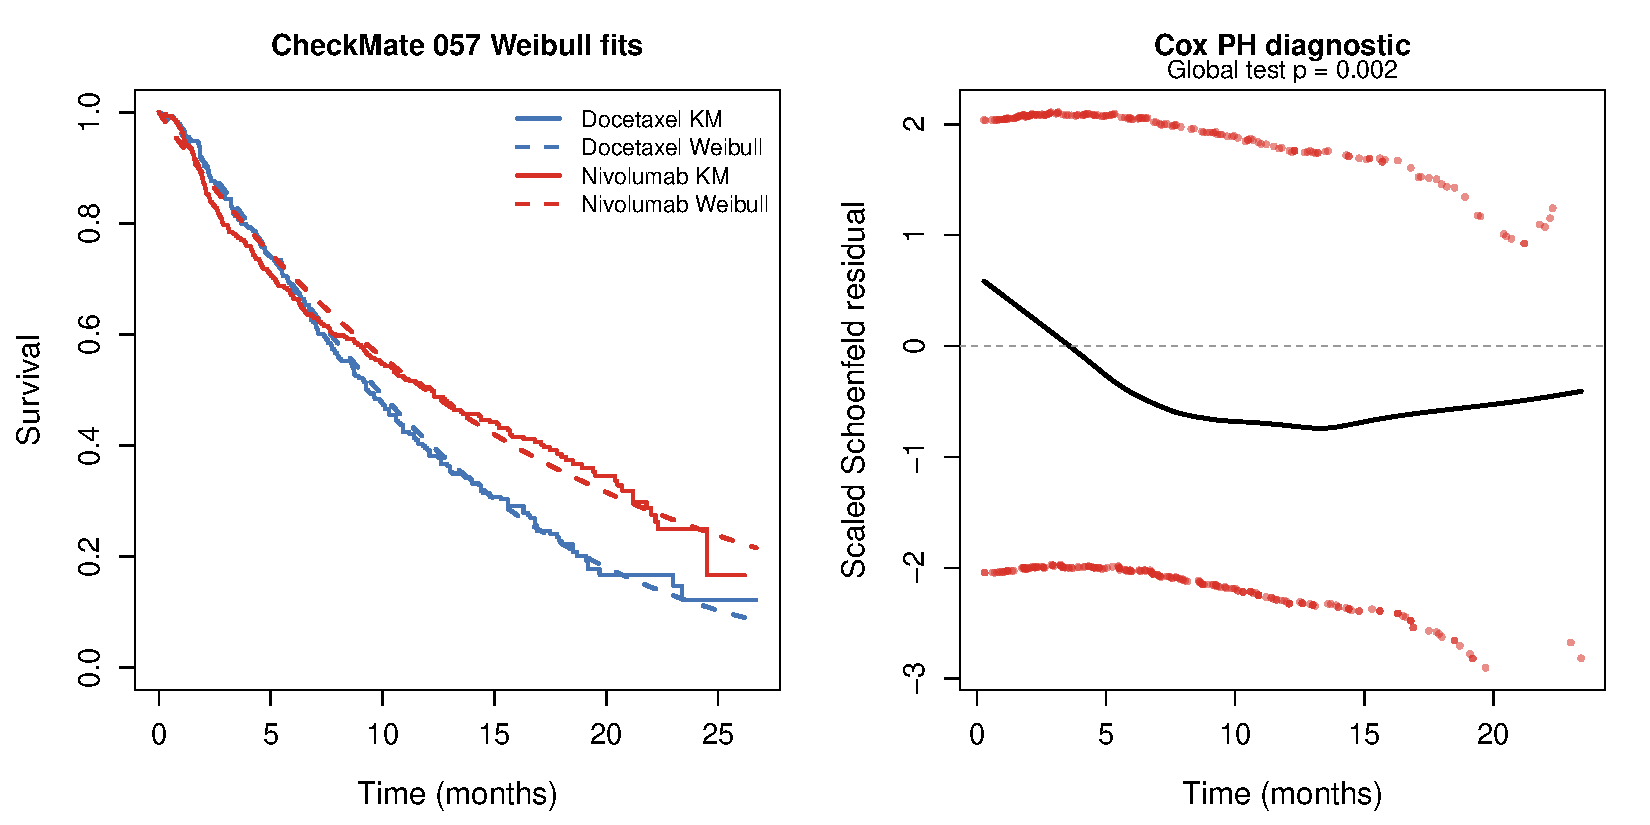
\includegraphics[width=0.95\textwidth]{output/figures/figure5-checkmate-diagnostics.pdf}
  \caption{Survival model fit (left) and proportional-hazards diagnostic (right)
    for the CheckMate 057 trial.}
  \label{fig:weibull}
  \label{fig:ph-diag}
  \label{fig:cm057-combined}
\end{figure}


In the docetaxel arm, $\kappa_0>1$ induces a monotone increasing hazard; in the nivolumab arm, $\kappa_1\approx1$ indicates an approximately constant hazard. The fitted log hazard ratio is time varying: $\alpha(1)=\AlphaCMOne$, it crosses zero near month \AlphaCMCross, and it reaches \AlphaCMTau\ at month \TauCM. This pattern is characteristic of immunotherapy and is consistent with the Schoenfeld diagnosis (Figure~\ref{fig:ph-diag}), whose negative residual slope indicates a decreasing log hazard ratio over time.

\paragraph{Choice of the censoring model}
Patients were enrolled from November 2012 through December 2013, and the
primary database lock occurred on March 18, 2015 \citep{Borghaei2015}.
For the fitted-design simulations, we represent staggered entry and follow-up
by administrative censoring $U\sim \mathrm{Uniform}(6,30)$ months.
Additionally, a small fraction of patients withdrew consent in the study or were lost to follow-up \citep{Borghaei2015}; we capture
this with light exponential dropout, $E \sim \mbox{Exp}(\lambda_c)$ with $\lambda_c = 0.005$/month (${\approx}6\%$ annually). The combined censoring time is $C = \min(E, U)$.
All three tests use $\tau=\TauCM$ months, corresponding to the clinically natural two-year overall survival landmark; Cox follow-up is administratively censored at the same horizon.



Table~\ref{tab:cm057-are-ere} presents the ARE and ERE results. Both measures yield the same ordering of the three tests:
\[
\RAH \ge \mathrm{Cox} \ge \DRMST.
\]
Figure~\ref{fig:cosine-cm057} presents the compass diagram for the CheckMate 057 data. The corresponding squared cosine similarities are
\[
\cos^2(\theta_{\mathrm{Cox}})=\CosSqCoxCM,\qquad
\cos^2(\theta_{\DRMST})=\CosSqDrmstCM,\qquad
\cos^2(\theta_{\RAH})=\CosSqRahCM.
\]
Because the ARE between two tests is given by the ratio of their squared cosine similarities, these values imply
\[
\mathrm{ARE}(\RAH/\mathrm{Cox})=\AreRahCoxCM
\quad\text{and}\quad
\mathrm{ARE}(\RAH/\DRMST)=\AreRahDrmstCM.
\]

Figure~\ref{fig:cosine-cm057} also provides a geometric explanation for why the crossing-hazards alternative favors the RAH-based test. The signal direction places substantial weight on the late follow-up period, where the treatment benefit of nivolumab is greatest. In contrast, the Cox test direction places relatively greater weight on earlier times and gradually decays over follow-up. The D-RMST test direction tapers more rapidly to zero as time approaches $\tau$, thereby placing even less weight on the late follow-up period. The RAH test direction, by comparison, is bounded below by $S_0(\tau)\approx\SzeroCMTau$, allowing it to retain meaningful weight at later times. Consequently, the RAH test direction is more closely aligned with the signal direction, resulting in greater efficiency under this crossing-hazards alternative.


\begin{table}[ht]
\centering
\caption{Theoretical ARE and empirical ERE under the CheckMate 057 fitted non-PH DGP; all methods use $\tau=24$ months, $n=300$ per arm, $B=500$.}
\label{tab:cm057-are-ere}
\begin{tabular}{lcc}
\toprule
Comparison & ARE & ERE
\\
\midrule
D-RMST/Cox & 0.915 & 0.935 \\
RAH/Cox & 1.199 & 1.332 \\
RAH/D-RMST & 1.310 & 1.425 \\
\bottomrule
\end{tabular}
\end{table}







\begin{figure}[ht]
  \centering
  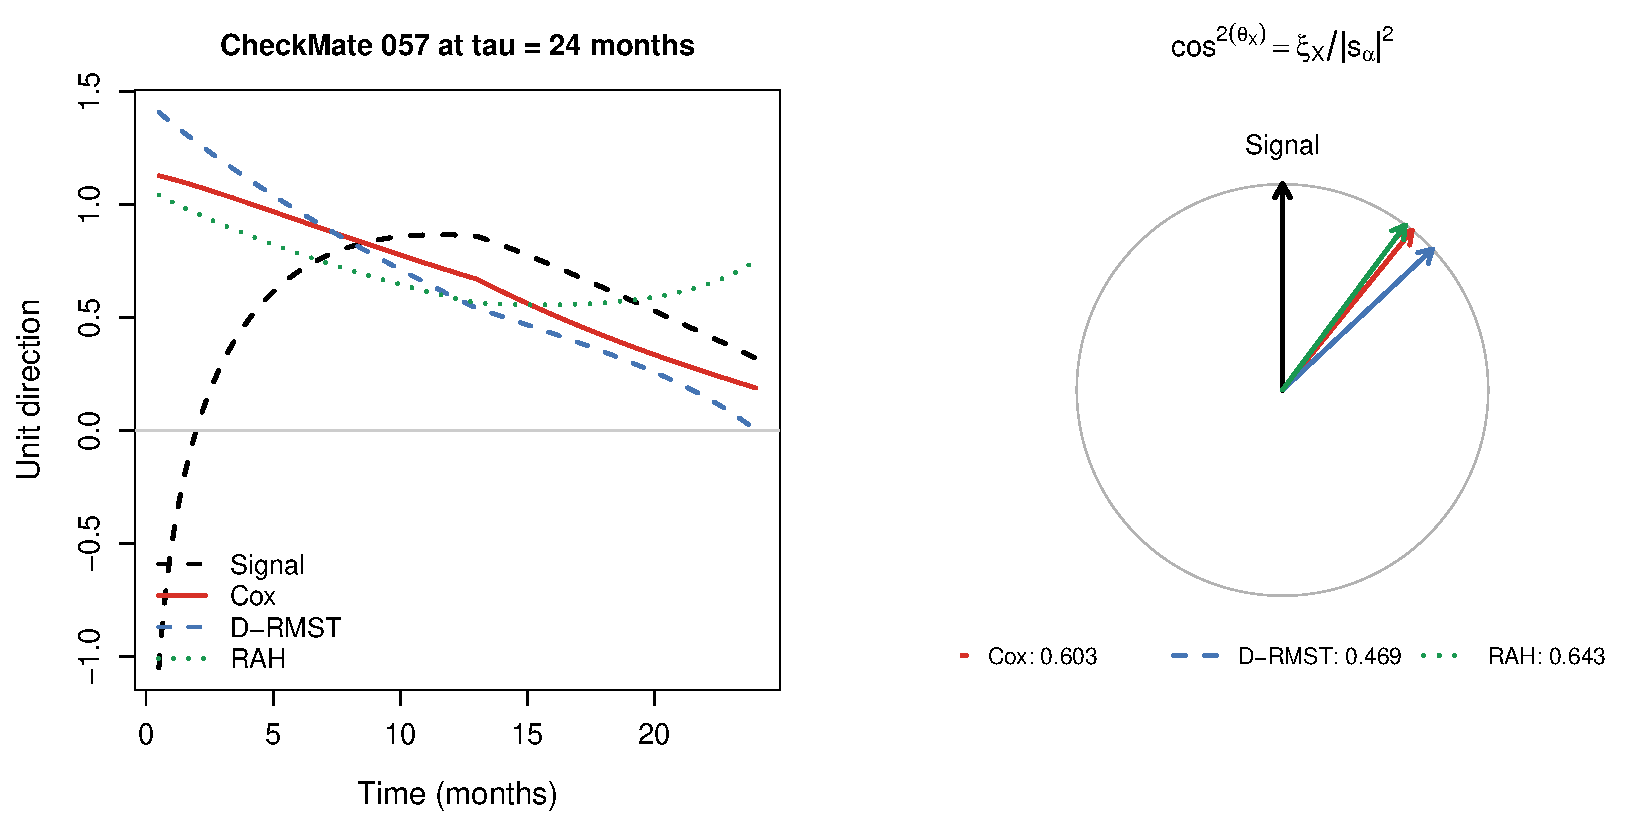
\includegraphics[width=0.90\linewidth]{output/figures/figure6-cosine-checkmate057.pdf}
  \caption{Unit-vector functions (left) and compass diagram (right)
  for Weibull distributions fitted to CheckMate 057 trial.
  All three tests use $\tau=\TauCM$ months; the function panel displays them on $[0,\tau]$.
  The signal direction is placed at 12 o'clock and reflects the
  crossing-hazards pattern. Each test direction is annotated with
  $\cos^2(\theta_X)$.
  RAH is closest to the signal direction, followed by Cox and D-RMST.}
  \label{fig:cosine-cm057}
\end{figure}

Beyond the efficiency metrics themselves, a key practical question is how differences in ARE translate into differences in power and required sample size. Figure~\ref{fig:power} shows the empirical power as a function of sample size per arm, with the RAH-based test consistently achieving the highest power, followed by the Cox model-based test and then the D-RMST-based test. Table~\ref{tab:cm057-power-n80} summarizes power at $n_0=n_1=300$ per arm and the first simulated sample size on the prespecified 50-patient grid to reach 80\% power. RAH reaches the target at \NPowerRahCM\ patients per arm, compared with \NPowerCoxCM\ for Cox and \NPowerDrmstCM\ for D-RMST. Thus, Cox and D-RMST require \NPowerCoxMorePct\% and \NPowerDrmstMorePct\% more patients than RAH, respectively, on this grid. At 300 patients per arm, empirical power is \PowerRahCMPct\% for RAH, \PowerCoxCMPct\% for Cox, and \PowerDrmstCMPct\% for D-RMST.



\begin{table}[ht]
\centering
\caption{Empirical power at $n=300$ per arm and first simulated sample size reaching 80\% power (50-patient grid, $B=2000$), with simulated, ARE-, and ERE-implied ratios relative to RAH.}
\label{tab:cm057-power-n80}
\begin{tabular}{lccccc}
\toprule
Method & Power & $n_{80}$ & Sim. ratio & ARE ratio & ERE ratio
\\
\midrule
Cox & 0.717 & 400 & 1.33 & 1.20 & 1.33 \\
D-RMST & 0.680 & 400 & 1.33 & 1.31 & 1.43 \\
RAH & 0.843 & 300 & 1.00 & 1.00 & 1.00 \\
\bottomrule
\end{tabular}
\end{table}

\begin{figure}[ht]
  \centering
  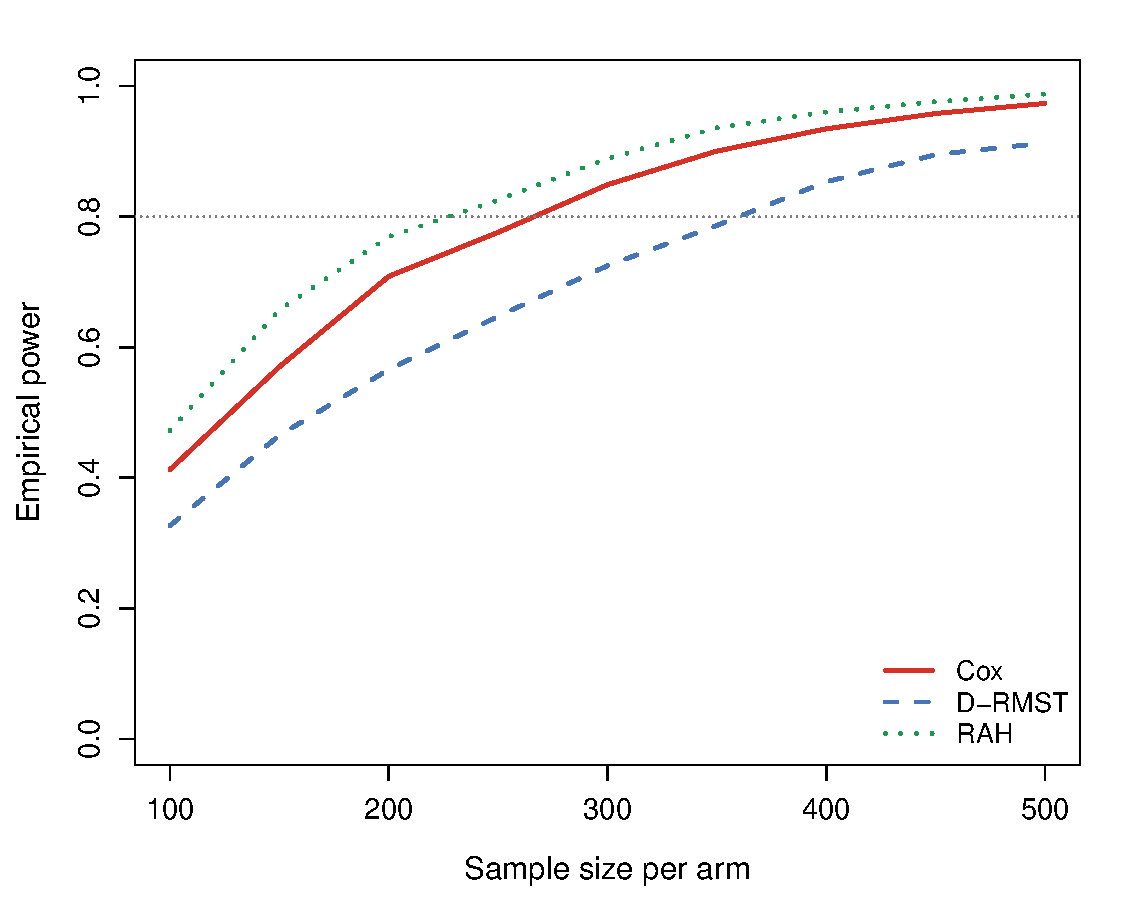
\includegraphics[width=0.65\textwidth]{output/figures/figure7-checkmate-power.pdf}
  \caption{Empirical power for Cox (red, solid), D-RMST (blue, dashed), and RAH (green, dotted) under the fitted CheckMate 057 non-PH alternative. Horizontal line: 80\% power.}
  \label{fig:power}
\end{figure}




We now assess the robustness of the ordering $\RAH \ge \rm{Cox} \ge \DRMST$
to the analysis horizon~$\tau$, dropout rate~$\lambda_c$, and assumed alternative. The results are reported in  Table~\ref{tab:sens-are}.
\begin{enumerate}
\item {\bf Horizon $\tau$:}
ARE(D-RMST/Cox) increases substantially with $\tau$, from \AreDrmstCMTauEighteen\ at $\tau=18$ to \AreDrmstCMTauTwentyfour\ at $\tau=24$. The relatively low efficiency of D-RMST at shorter horizons reflects truncation of the late treatment benefit. In contrast, ARE(RAH/Cox) is comparatively stable (\AreRahCMTauEighteen, \AreRahCMTauTwentyone, and \AreRahCMTauTwentyfour\ at 18, 21, and 24 months), while ARE(RAH/D-RMST) decreases from \AreRahDrmstCMTauEighteen\ to \AreRahDrmstCMTauTwentyfour.

\item {\bf Dropout rate:}
Increasing $\lambda_c$ from 0.001 to 0.020 shifts ARE(D-RMST/Cox) from \AreDrmstCMDropoutLow\ to \AreDrmstCMDropoutHigh, indicating that heavier dropout reduces the relative efficiency of Cox. ARE(RAH/Cox) increases modestly from \AreRahCMDropoutLow\ to \AreRahCMDropoutHigh, whereas ARE(RAH/D-RMST) decreases from \AreRahDrmstCMDropoutLow\ to \AreRahDrmstCMDropoutHigh. This pattern reflects the growing attenuation of the Cox weight at later times as $S_C(t)$ decreases.

\item {\bf PH vs.\ non-PH:}
Under a PH alternative (HR$=0.75$, with the same Weibull shape as for docetaxel), Cox is the most efficient, with ARE(D-RMST/Cox)$=\AreDrmstCMPH$ and ARE(RAH/Cox)$=\AreRahCMPH$. This highlights that RAH's advantage in the fitted non-PH setting arises from its greater alignment with the late treatment benefit; the positive weight floor provides no such advantage under PH.
\end{enumerate}

In summary, the ERE and ARE results are generally consistent. Under the assumed non-PH alternative, the RAH-based test is more efficient than both Cox model-based and D-RMST-based tests. Under the PH alternative, however, the RAH-based test is slightly less efficient than the Cox model-based test.

\begin{table}[ht]
\centering
\caption{Sensitivity to analysis horizon, dropout rate, and hazard structure; the common baseline is $\tau=24$, $\lambda_c=0.005$, fitted non-PH, $n=300$ per arm and $B=500$.}
\label{tab:sens-are}
\resizebox{\textwidth}{!}{
\begin{tabular}{lccccccc}
\toprule
Panel & Setting & ARE(D/C) & ARE(R/C) & ARE(R/D) & ERE(D/C) & ERE(R/C) & ERE(R/D)
\\
\midrule
Horizon & $\tau=18$ & 0.651 & 1.198 & 1.841 & 0.607 & 1.292 & 2.127 \\
Horizon & $\tau=21$ & 0.789 & 1.211 & 1.533 & 0.768 & 1.299 & 1.691 \\
Horizon & $\tau=24$ & 0.915 & 1.199 & 1.310 & 0.935 & 1.332 & 1.425 \\
Dropout & $\lambda_c=0.001$ & 0.884 & 1.180 & 1.335 & 0.895 & 1.223 & 1.367 \\
Dropout & $\lambda_c=0.005$ & 0.915 & 1.199 & 1.310 & 0.935 & 1.332 & 1.425 \\
Dropout & $\lambda_c=0.020$ & 1.039 & 1.265 & 1.217 & 1.071 & 1.369 & 1.278 \\
Hazard & Non-PH (fitted) & 0.915 & 1.199 & 1.310 & 0.935 & 1.332 & 1.425 \\
Hazard & PH (HR$=0.75$) & 0.995 & 0.870 & 0.875 & 0.990 & 0.904 & 0.913 \\
\bottomrule
\end{tabular}
}
\end{table}


\section{Discussion}
\label{sec:discussion}


This paper makes three contributions: it characterizes the efficiency of the recently proposed RAH-based test, provides a cosine metric that places the Cox-, D-RMST-, and RAH-based tests on a common geometric scale, and shows how censoring and accrual shape which test is preferred at the design stage. The main message is that no single test uniformly dominates; rather, the most efficient test depends jointly on the underlying pattern of treatment effect and the censoring distribution. The Cox model-based test is most efficient under the PH assumption. The D-RMST-based test is particularly well suited for detecting fading treatment effects, as it places greater weight on early survival differences. In contrast, the RAH-based test is particularly attractive for detecting delayed treatment benefits, a pattern that has been repeatedly observed in studies of immunotherapy in oncology. In addition, the censoring and accrual designs can substantially affect the relative performance of these tests. These effects can be readily visualized through the proposed cosine metrics, which quantify the alignment between the underlying treatment-effect signal and the directions targeted by each test. In practice, the cosine metric is best used to compare candidate tests across a range of plausible scenarios rather than to commit to one in advance in the study design.








Several extensions are natural. The cosine metric could be used as an objective function for optimizing accrual and follow-up duration, rather than merely as a diagnostic for comparing prespecified tests. In addition, because $W_{\RAH}$ is not a Fleming--Harrington weight \citep{FlemingHarrington1991}, incorporating it alongside $W_{\mathrm{Cox}}$ and $W_{\DRMST}$ in a Max-combo test would broaden the class of treatment-effect alternatives that can be effectively detected.


\appendix

\section{Asymptotic Distribution of the RAH Statistic}
\label{sec:appendix-proofs}

\subsection{Local-alternative drift}
Throughout we work under \emph{Pitman contiguous alternatives}:
\begin{equation}\label{eq:local-alt}
  H_{An}:\quad
  \log\frac{\lambda_{1n}(t)}{\lambda_0(t)}=\frac{\alpha(t)}{\sqrt{n}},
\end{equation}
where $\alpha(\cdot)$ is a fixed function on $(0,\tau]$.
Under~\eqref{eq:local-alt}, to first order in $n^{-1/2}$:
$\sqrt{n}[S_{1n}(t)-S_0(t)]\to-S_0(t)\int_0^t\lambda_0(u)\alpha(u)\dd u$.

\begin{proposition}\label{prop:mean-rah}
Under $H_{An}$, $\sqrt{n}\log(\hat\theta_{\RAH})$ is asymptotically normal
with mean
\begin{equation}\label{eq:mean-RAH-compact}
  \mu_{\RAH}
    =\int_0^\tau
       \!\left[\frac{1}{F_0(\tau)}-\frac{R_0(t)}{R_0(\tau)}\right]
       \alpha(t)\lambda_0(t)\dd t.
\end{equation}
\end{proposition}

\begin{proof}
 $\sqrt{n}\log(\hat\theta_{\RAH})=U_n+V_n$,
where $U_n=\sqrt{n}[\log\hat F_1(\tau)-\log\hat F_0(\tau)]$
and $V_n=-\sqrt{n}[\log\hat R_1(\tau)-\log\hat R_0(\tau)]$.
Next, we have
\begin{align*}
  U_n &= F_0(\tau)^{-1}\sqrt{n}[\hat F_1-\hat F_0](\tau)+o_p(1)\\
      &=F_0(\tau)^{-1}\sqrt{n}[F_1-F_0](\tau)-F_0(\tau)^{-1}\sqrt{n}[(\hat S_1- S_1)-(\hat S_0-S_0)](\tau)+o_p(1)\\
      &=\int_0^\tau\frac{S_0(\tau)}{F_0(\tau)}\alpha(t)\lambda_0(t)\dd t+\eta_{1n}+o_p(1),
\end{align*}
and
\begin{align*}
V_n &= -R_0(\tau)^{-1}\int_0^\tau\sqrt{n}[\hat S_1(t)-\hat S_0(t)]\dd t +o_p(1)\\
    &= -R_0(\tau)^{-1}\int_0^\tau\sqrt{n}[S_1(t)-S_0(t)]\dd t -R_0(\tau)^{-1}\int_0^\tau\sqrt{n}\left[(\hat{S}_1-S_1)-(\hat{S}_0-S_0)\right](t)\dd t+o_p(1)\\
    &=R_0(\tau)^{-1}\int_0^\tau S_0(t)A(t)\dd t+\eta_{2n}+o_p(1),
\end{align*}
where $A(t)=\int_0^t\lambda_0(u)\alpha(u)\dd u$ and $(\eta_{1n}, \eta_{2n})'$ converging in distribution to a mean zero bivariate Gaussian distribution as $n\to \infty.$  Furthermore,
\[R_0(\tau)^{-1}\int_0^\tau S_0(t) A(t)\dd t=A(\tau)-\int_0^\tau\lambda_0(t)\alpha(t) \frac{R_0(t)}{R_0(\tau)}\dd t=\int_0^\tau \left[1-\frac{R_0(t)}{R_0(\tau)}\right]\alpha(t)\lambda_0(t)dt.\]
Substituting and simplifying gives~\eqref{eq:mean-RAH-compact}.
\end{proof}

\subsection{Pitman efficacy of RAH-based test}
\label{sec:appendix-pitman}
The Pitman efficacy formula follows from $\xi_{\RAH}=\mu_{\RAH}^2/\sigma_{\RAH}^2$:
\begin{equation}\label{eq:eff-RAH}
  \xi_{\RAH}
    =\frac{\displaystyle
      \left[\int_0^\tau\!\left\{\dfrac{1}{F_0(\tau)}-\dfrac{R_0(t)}{R_0(\tau)}\right\}
            \alpha(t)\lambda_0(t)\dd t\right]^{\!2}}{
      \displaystyle
      \int_0^\tau\!\left\{\dfrac{1}{F_0(\tau)}-\dfrac{R_0(t)}{R_0(\tau)}\right\}^{\!2}
      \dfrac{\lambda_0(t)}{w(t)}\dd t}.
\end{equation}
The efficacies of Cox and D-RMST follow from \citet{Tian2018}:
\begin{equation}\label{eq:eff-Cox}
  \xi_{\mathrm{Cox}}
    =\frac{\displaystyle
       \left[\int_0^{\tau} w(t)\,\alpha(t)\lambda_0(t)\dd t\right]^2}{
      \displaystyle
       \int_0^{\tau} w(t)\,\lambda_0(t)\dd t},
\end{equation}
\begin{equation}\label{eq:eff-DRMST}
  \xi_{\DRMST}
    =\frac{\displaystyle
       \left[\int_0^{\tau}\!\left\{R_0(\tau)-R_0(t)\right\}
             \alpha(t)\lambda_0(t)\dd t\right]^2}{
      \displaystyle
       \int_0^{\tau}\!\left\{R_0(\tau)-R_0(t)\right\}^{\!2}
       \frac{\lambda_0(t)}{w(t)}\dd t}.
\end{equation}



\section{Derivation of the Weight Function Representations}
\label{sec:appendix-weights}

We prove that each of the three statistics of
Section~\ref{sec:three-stats} is asymptotically equivalent to a version of
weighted logrank statistic~\eqref{eq:wlr-generic},
$$\int_0^\tau W(t)\,d[\hat\Lambda_1(t)-\hat\Lambda_0(t)].$$
All derivations use: (i) the KM linear representation
$$\sqrt{n}(\hat S_k-S_k)=-S_k\sqrt{n}(\hat\Lambda_k-\Lambda_k)+o_p(1);$$
(ii)  the functional delta method; and
(iii) the local-alternative approximation
$$S_{1n}(t)=S_0(t)-\frac{S_0(t)A(t)}{\sqrt{n}}+o(n^{-1/2}).$$
For simplicity, we also assume equal allocation and common censoring $S_C(\cdot)$.

\begin{itemize}
\item \textbf{Cox model-based statistic.}
  Let
\(\ell_n(\theta)\) be the log partial likelihood over \([0, \tau]\),
\(U_n(\theta)=\partial\ell_n(\theta)/\partial\theta\) its score, and
\(\mathcal I_n(\theta)=-\partial^2\ell_n(\theta)/\partial\theta^2\) the
observed information.  The score at \(\theta=0\) is exactly the log-rank
statistic, \(n^{-1}U_n(0)=U_{\mathrm{Cox}}\) in ~\eqref{eq:cox-stat}, and
\[
  n^{-1}\mathcal I_n(0)
    \;\longrightarrow\;
  \int_0^{\tau}w(t)\lambda_0(t)dt=\sigma_\theta^{-2}
\]
in probability, uniformly in a neighbourhood of \(\theta=0\).  Since
\(\hat\theta=O_p(n^{-1/2})\) under the local
alternatives~\eqref{eq:local-alt} and \(U_n(\hat\theta)=0\), a one-term
Taylor expansion of \(U_n(\theta)\) about \(\theta=0\) gives
\[
  0=n^{-1}U_n(\hat\theta)
   =U_{\mathrm{Cox}}-n^{-1}\mathcal I_n(0)\,\hat\theta+o_p(n^{-1/2})
  \Rightarrow
  \sqrt n\,\hat\theta=\sigma_\theta^{2}\sqrt n\,U_{\mathrm{Cox}}+o_p(1).
\]
Hence \(\sqrt n\,\hat\theta=\sigma_\theta^2\sqrt n\,U_{\mathrm{Cox}}+o_p(1)\), and \(Z_{\mathrm{Cox}}\) and the normalized log-rank statistic are
asymptotically equivalent.  The logrank statistic~\eqref{eq:cox-stat} is
already of the weighted-log-rank form, with random weight
\[
 \hat{w}_{\rm{Cox}}(t)=\frac{Y_1(t)Y_0(t)}{Y_1(t)+Y_0(t)},
\]
where $Y_k(t)$ is the size of the risk set of group $k$ at $t.$  By law of large numbers, $n^{-1}\hat{w}_{\rm{Cox}}(t)$ converges to \(w(t)\), which is $S_0(t)S_C(t)/4$ under equal
allocation and common censoring. Therefore, we can set
\[
  W_{\mathrm{Cox}}(t)=4w(t)=\;S_0(t)S_C(t),
\]
in (\ref{eq:wlr-generic}).


\item \textbf{D-RMST.}
By functional delta-method, we have
\begin{align*}
  \sqrt{n}\hat\theta_{\DRMST}&=-\sqrt{n}\int_0^\tau S_0(t)\,\hat{\Delta}_\Lambda(t)\dd t+O\bigl(\sqrt{n}\|\hat{\Delta}_\Lambda\|^2\bigr)\\
  &=-\sqrt{n}\int_0^\tau S_0(t)\int_0^t d\hat{\Delta}_\Lambda(u)\dd t+O_p\bigl(n^{-1/2}\bigr)\\
  &=-\sqrt{n}\int_0^\tau\left\{\int_u^\tau S_0(t)\dd t\right\}d\hat{\Delta}_\Lambda(u)+O_p\bigl(n^{-1/2}\bigr)\\
  &=-\sqrt{n}\int_0^\tau\{R_0(\tau)-R_0(u)\}\,d\hat{\Delta}_\Lambda(u)+o_p(1).
\end{align*}
Therefore, we may set the weight as
\[
  W_{\DRMST}(t)=\frac{R_0(\tau)-R_0(t)}{R_0(\tau)},
\]
as $Z_{\DRMST}$ is invariant to multiplying any nonzero constant to the weight function.


\item \textbf{RAH.}
Using the same argument together with the delta method for $\log F_k(\tau)$ and $\log R_k(\tau)$,
\[
\log\hat\theta_{\RAH}=\int_0^\tau\left[\frac{S_0(\tau)}{F_0(\tau)}+\frac{R_0(\tau)-R_0(t)}{R_0(\tau)}\right]d\hat\Delta_\Lambda(t)+O_p(n^{-1}).
\]
Multiplying by $F_0(\tau)>0$ gives the equivalent weight
\[
  W_{\RAH}(t)
    =S_0(\tau)+F_0(\tau)\,\frac{R_0(\tau)-R_0(t)}{R_0(\tau)}
    =S_0(\tau)+\bigl[1-S_0(\tau)\bigr]\, W_{\DRMST}(t).
\]
\end{itemize}

\section{Simulation Study for PH Setting at HR\,=\,0.82}
\label{sec:appendix-hr082}

We repeat the simulation for PH scenarios with HR=0.82. The results are reported in Tables~\ref{tab:sim3a-hr082} and~\ref{tab:sim3c-hr082}.
Both ARE and ERE are similar to to those for HR$=0.70$:

\begin{table}[ht]
\centering
\caption{ARE and ERE under PH (HR$=0.82$), $\kappa=0.826$, $\tau=40$, $n=400$ per arm, $B=2000$.}
\label{tab:sim3a-hr082}
\resizebox{\textwidth}{!}{
\begin{tabular}{lccccccc}
\toprule
Censoring & $S_0(40)$ & ARE(D/C) & ARE(R/C) & ARE(R/D) & ERE(D/C) & ERE(R/C) & ERE(R/D)
\\
\midrule
Light & 0.10 & 0.994 & 0.941 & 0.947 & 1.001 & 0.939 & 0.938 \\
Light & 0.20 & 0.980 & 0.917 & 0.935 & 0.987 & 0.898 & 0.910 \\
Light & 0.30 & 0.967 & 0.898 & 0.929 & 0.968 & 0.911 & 0.942 \\
Light & 0.40 & 0.954 & 0.883 & 0.926 & 0.957 & 0.872 & 0.911 \\
Light & 0.50 & 0.942 & 0.871 & 0.924 & 0.929 & 0.885 & 0.953 \\
Light & 0.60 & 0.931 & 0.860 & 0.924 & 0.958 & 0.852 & 0.889 \\
Light & 0.70 & 0.920 & 0.851 & 0.924 & 0.930 & 0.839 & 0.903 \\
Light & 0.80 & 0.911 & 0.842 & 0.925 & 0.952 & 0.831 & 0.872 \\
Light & 0.90 & 0.901 & 0.835 & 0.927 & 0.913 & 0.834 & 0.914 \\
\midrule
Heavy & 0.10 & 0.982 & 0.798 & 0.812 & 0.989 & 0.727 & 0.735 \\
Heavy & 0.20 & 0.993 & 0.751 & 0.756 & 1.001 & 0.718 & 0.717 \\
Heavy & 0.30 & 0.997 & 0.720 & 0.722 & 1.004 & 0.704 & 0.701 \\
Heavy & 0.40 & 0.998 & 0.698 & 0.699 & 1.004 & 0.689 & 0.686 \\
Heavy & 0.50 & 0.998 & 0.680 & 0.682 & 1.007 & 0.672 & 0.667 \\
Heavy & 0.60 & 0.997 & 0.666 & 0.668 & 1.001 & 0.676 & 0.675 \\
Heavy & 0.70 & 0.995 & 0.654 & 0.658 & 0.996 & 0.685 & 0.688 \\
Heavy & 0.80 & 0.992 & 0.644 & 0.649 & 0.993 & 0.661 & 0.665 \\
Heavy & 0.90 & 0.990 & 0.635 & 0.642 & 1.054 & 0.698 & 0.662 \\
\bottomrule
\end{tabular}
}
\end{table}

\begin{table}[ht]
\centering
\caption{ARE, power, and ERE under PH (HR$=0.82$), $S_0(40)=0.50$, $\tau=40$, $n=400$ per arm, $B=2000$.}
\label{tab:sim3c-hr082}
\resizebox{\textwidth}{!}{
\begin{tabular}{lcccccccccc}
\toprule
Censoring & $\kappa$ & ARE(D/C) & ARE(R/C) & ARE(R/D) & Power C & Power D & Power R & ERE(D/C) & ERE(R/C) & ERE(R/D)
\\
\midrule
Light & 0.500 & 0.962 & 0.922 & 0.959 & 0.458 & 0.452 & 0.433 & 0.980 & 0.918 & 0.937 \\
Light & 0.826 & 0.942 & 0.871 & 0.924 & 0.435 & 0.418 & 0.395 & 0.929 & 0.885 & 0.953 \\
Light & 1.000 & 0.934 & 0.844 & 0.904 & 0.448 & 0.406 & 0.393 & 0.941 & 0.838 & 0.891 \\
Light & 1.500 & 0.919 & 0.781 & 0.850 & 0.415 & 0.382 & 0.341 & 0.931 & 0.802 & 0.862 \\
Light & 2.000 & 0.914 & 0.737 & 0.806 & 0.383 & 0.349 & 0.307 & 0.906 & 0.765 & 0.844 \\
\midrule
Heavy & 0.500 & 0.996 & 0.750 & 0.753 & 0.376 & 0.379 & 0.307 & 1.003 & 0.744 & 0.741 \\
Heavy & 0.826 & 0.998 & 0.680 & 0.682 & 0.336 & 0.337 & 0.260 & 1.007 & 0.672 & 0.667 \\
Heavy & 1.000 & 0.998 & 0.653 & 0.654 & 0.298 & 0.301 & 0.237 & 0.996 & 0.632 & 0.635 \\
Heavy & 1.500 & 0.994 & 0.599 & 0.603 & 0.277 & 0.284 & 0.224 & 0.991 & 0.632 & 0.638 \\
Heavy & 2.000 & 0.991 & 0.570 & 0.576 & 0.247 & 0.253 & 0.183 & 0.995 & 0.584 & 0.587 \\
\bottomrule
\end{tabular}
}
\end{table}

\section{Simulation Study for PH Setting with Different Sample Size, Horizon and Survival Distributions}
\label{sec:appendix-tau10}

We also repeat simulation study the PH setting under different design:
$\tau=10$, $n_0=n_1=150$, and three baseline distributions (
an exponential with $S_0(10)\approx0.37$;
a Weibull baseline with a
decreasing hazard ($\kappa=0.7$) and $S_0(10)=0.5;$ and a Weibull baseline with an increasing hazard ($\kappa=1.5$) and $S_0(10)=0.5.$)
We also consider light censoring with $C \sim \min \left\{U(8, 12), \mbox{Exp}(0.02)\right\}$ and heavy censoring with $C\sim \min \left\{U(8, 12), \mbox{Exp}(0.20)\right\}$.

The results are reported in Table~\ref{tab:sim-tau10}. RAH is more efficient than D-RMST under light censoring, whereas D-RMST is substantially more efficient than RAH under heavy censoring.

\begin{table}[ht]
\centering
\caption{ARE and ERE under PH (HR$=0.70$), $\tau=10$, $n=150$ per arm, $B=500$.}
\label{tab:sim-tau10}
\resizebox{\textwidth}{!}{
\begin{tabular}{lccccccc}
\toprule
Censoring & Baseline & ARE(D/C) & ARE(R/C) & ARE(R/D) & ERE(D/C) & ERE(R/C) & ERE(R/D)
\\
\midrule
Light & Weibull(kappa=0.7) & 0.920 & 0.981 & 1.067 & 0.985 & 0.974 & 0.989 \\
Light & Exponential(lambda0=0.10) & 0.913 & 0.976 & 1.068 & 0.941 & 0.989 & 1.051 \\
Light & Weibull(kappa=1.5) & 0.853 & 0.954 & 1.119 & 0.895 & 0.906 & 1.013 \\
\midrule
Heavy & Weibull(kappa=0.7) & 0.970 & 0.669 & 0.690 & 1.025 & 0.722 & 0.704 \\
Heavy & Exponential(lambda0=0.10) & 0.973 & 0.665 & 0.684 & 1.033 & 0.670 & 0.648 \\
Heavy & Weibull(kappa=1.5) & 0.987 & 0.651 & 0.659 & 0.976 & 0.611 & 0.626 \\
\bottomrule
\end{tabular}
}
\end{table}

\section{Additional Simulations: Crossing Hazards}
\label{sec:appendix-crossing}



In this simulation, $\alpha(t)=\log(0.46)+(t/t_M)$ with $t_M=43$ months,
$\kappa=0.826$, and $S_0(40)=0.50$: the HR starts at $0.46,$ crosses one, and rises above 1 late in follow-up. Thus, an early treatment benefit is reversed to harm at late times.
Table~\ref{tab:sim-crossing} reports the ARE and ERE under light and heavy censoring. D-RMST is more efficient than Cox, whereas RAH is less efficient than both Cox and D-RMST, under both censoring regimes. The efficiency separation is larger under heavy censoring.




\begin{table}[ht]
\centering
\caption{ARE and ERE under crossing hazards; $t_M=43$, $\tau=40$, $S_0(40)=0.50$, $n=400$ per arm, $B=2000$.}
\label{tab:sim-crossing}
\begin{tabular}{lcccccc}
\toprule
Cens. & ARE(D/C) & ARE(R/C) & ARE(R/D) & ERE(D/C) & ERE(R/C) & ERE(R/D)
\\
\midrule
Light & 1.193 & 0.683 & 0.573 & 1.272 & 0.599 & 0.471 \\
\midrule
Heavy & 1.016 & 0.429 & 0.422 & 1.060 & 0.374 & 0.353 \\
\bottomrule
\end{tabular}
\end{table}













\bibliographystyle{plainnat}
\bibliography{manuscript/refs}
\end{document}